% !TEX TS-program = pdflatex
% !TEX encoding = UTF-8 Unicode

% This is a simple template for a LaTeX document using the "article" class.
% See "book", "report", "letter" for other types of document.

\documentclass[11pt]{article} % use larger type; default would be 10pt

\usepackage[utf8]{inputenc} % set input encoding (not needed with XeLaTeX)

%%% Examples of Article customizations
% These packages are optional, depending whether you want the features they provide.
% See the LaTeX Companion or other references for full information.

%%% PAGE DIMENSIONS
\usepackage{geometry} % to change the page dimensions
\geometry{a4paper} % or letterpaper (US) or a5paper or....
% \geometry{margin=2in} % for example, change the margins to 2 inches all round
% \geometry{landscape} % set up the page for landscape
%   read geometry.pdf for detailed page layout information

\usepackage{graphicx} % support the \includegraphics command and options

% \usepackage[parfill]{parskip} % Activate to begin paragraphs with an empty line rather than an indent

%%% PACKAGES
\usepackage{booktabs} % for much better looking tables
\usepackage{array} % for better arrays (eg matrices) in maths
\usepackage{paralist} % very flexible & customisable lists (eg. enumerate/itemize, etc.)
\usepackage{verbatim} % adds environment for commenting out blocks of text & for better verbatim
\usepackage{subfig} % make it possible to include more than one captioned figure/table in a single float
% These packages are all incorporated in the memoir class to one degree or another...

\usepackage[hidelinks]{hyperref} % for links in citations

\usepackage{todonotes} % for draft notes

% MATH PACKAGES
\usepackage{amsmath}
\usepackage{amssymb}

% CHEM PACKAGES
\usepackage{mhchem}


%%% HEADERS & FOOTERS
\usepackage{fancyhdr} % This should be set AFTER setting up the page geometry
\pagestyle{fancy} % options: empty , plain , fancy
\renewcommand{\headrulewidth}{0pt} % customise the layout...
\lhead{}\chead{}\rhead{}
\lfoot{}\cfoot{\thepage}\rfoot{}

%%% SECTION TITLE APPEARANCE
\usepackage{sectsty}
\allsectionsfont{\sffamily\mdseries\upshape} % (See the fntguide.pdf for font help)
% (This matches ConTeXt defaults)

%%% ToC (table of contents) APPEARANCE
\usepackage[nottoc,notlof,notlot]{tocbibind} % Put the bibliography in the ToC
\usepackage[titles,subfigure]{tocloft} % Alter the style of the Table of Contents
\renewcommand{\cftsecfont}{\rmfamily\mdseries\upshape}
\renewcommand{\cftsecpagefont}{\rmfamily\mdseries\upshape} % No bold!


%%% END Article customizations

%%% The "real" document content comes below...

\title{HomologyRing: A Python Tool for Analyzing Intra- and Inter-Chain Contact Specificity in Protein Families}
\author{Tanner Aaron Graves}
%\date{} % Activate to display a given date or no date (if empty),
         % otherwise the current date is printed 
% Supervisor Daminano Piovisan
% Department of Mathematics
% Graduation Date
% Degree Information : Masters of Science: Data Science
% Department of Mathematics


\begin{document}
\maketitle

\begin{abstract}
Contacts formed by peptides are principally responsible for stabilizing protein structure and determining protein function. AlphaFold 2, developed by DeepMind has proven capable of predicting protein structure with unprecedented accuracy. With predictions available for the majority of known proteins, AlphaFold has proven transformative for bioinformatics, resulting in an abundance of high-quality structural data. RING is a software that deterministically predicts non-covalent interactions in such structure files, providing high accuracy contact information with a wide verity of uses including: aiding in human understanding of protein structure or function, and training machine learning models. HomologyRing is a Python package that combines the functionality of RING with a homology search, enabling the analysis of contact conservation and variance across many of evolutionarily related proteins. Starting from a query structure or sequence, HomologyRing uses BLAST to perform a homology search against either UniProt or Protein Data Bank (PDB) databases, and subsequently using RING to collect contact information for corresponding AlphaFold or PDB structures. We demonstrate the utility of the resulting homology-enriched contact information for characterizing how preservation and variance of contacts in homologs contributes to protein structure, function, and partner binding. By mapping contacts to corresponding residues in a multiple sequence alignment (MSA), HomologyRing compiles and visualizes detailed information on intra- and inter-chain contacts, with wide potential applications, including: study of DNA, ligand, and partner binding specificity. 
\end{abstract}

\newpage
\tableofcontents
\newpage

\section*{Abbreviations and Terminology}

\begin{tabbing}
	Abbreviation \hspace{2cm} \= Definition \\
	\textbf{MSA} \> Multiple Sequence Alignment \\
	\textbf{RIN} \> Residue Interaction Network \\
	\textbf{hRIN} \> Homology Residue Interaction Network \\
	\textbf{PDB} \> Protein Data Bank \\
	\textbf{RING} \> Residue Interaction Network Generator \cite{ring}\\
\end{tabbing}
We interchangeably use the following terms depending on context: \emph{interaction}, \emph{non-covalent interaction}, and \emph{edge}.\\
Types of non-covalent interactions are referred to by RING identifiers. A complete list of which can be found in Appendix  \ref{appendix:RING-inter}\\

\section{Introduction}
This section assumes familiarity with central biological dogma, as well as knowledge of basic concepts in Bioinformatics. Extensive background is provided in Appendix \ref{appendix:bio-background} that aims to accomidate readers of various backgrounds. The topics particularly relevant to this work are explained in the following sections. 

\section{Biological Background}
\label{appendix:bio-background}
\subsection{Central Dogma}
Amino acids, different properties
Proteins transcribed from genes - DNA that codes 

\subsection{Protein Folding}
Proteins are fundamentally polymers, or variable length chains of amino acid units joined together by covalent bonds.
The individual amino acids in a chain are referred to as residues. 
They all have two primary componets: a backbone consisting of a central carbon atom with two essential groups on oppsite sides: an \ce{-NH_2} amino gorup and a  \ce{-COOH} carboxyl group; and a variable side chain that is principally responsible for the physical and chemical properties of the residue.
\begin{figure}[ht] % replace with [H} if position is causing problems.
    \centering
    %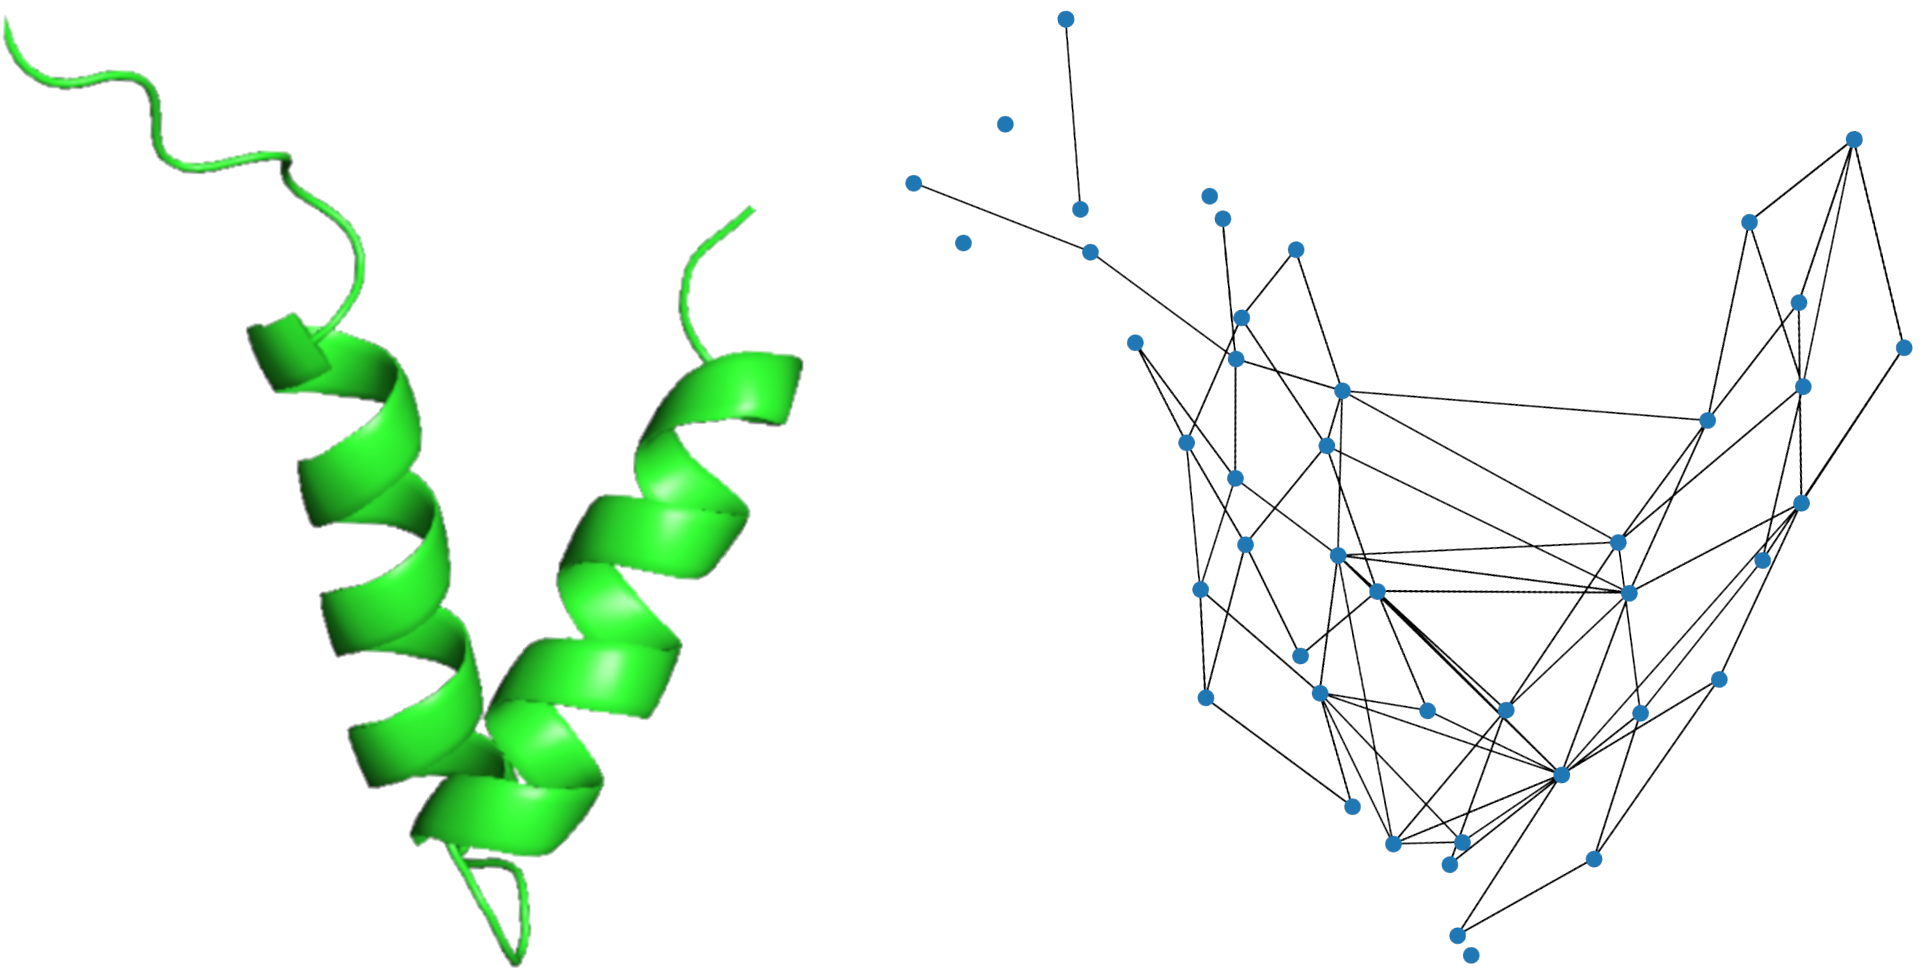
\includegraphics[width=0.5\textwidth]{fig/chain_to_RIN.png}
    \caption{Example of an amino acid structure.}
    \label{fig:AA-prop}
\end{figure}
Proteins are bonded together in a chain by forming peptide bonds --- a perticular kind of covalent bond where the amino group of one residue will bond to the carboxyl group of another. The sequence of the spesific residues in a protein chain is referred to as the \emph{primary structure} of a protein. 

There are 20 standard amino acids that primarly differ by their side chains. These side chains have varying polarity, charge, and size which effects the chemical and physical properties of the residue.

\begin{figure}[ht] % replace with [H} if position is causing problems.
    \centering
    %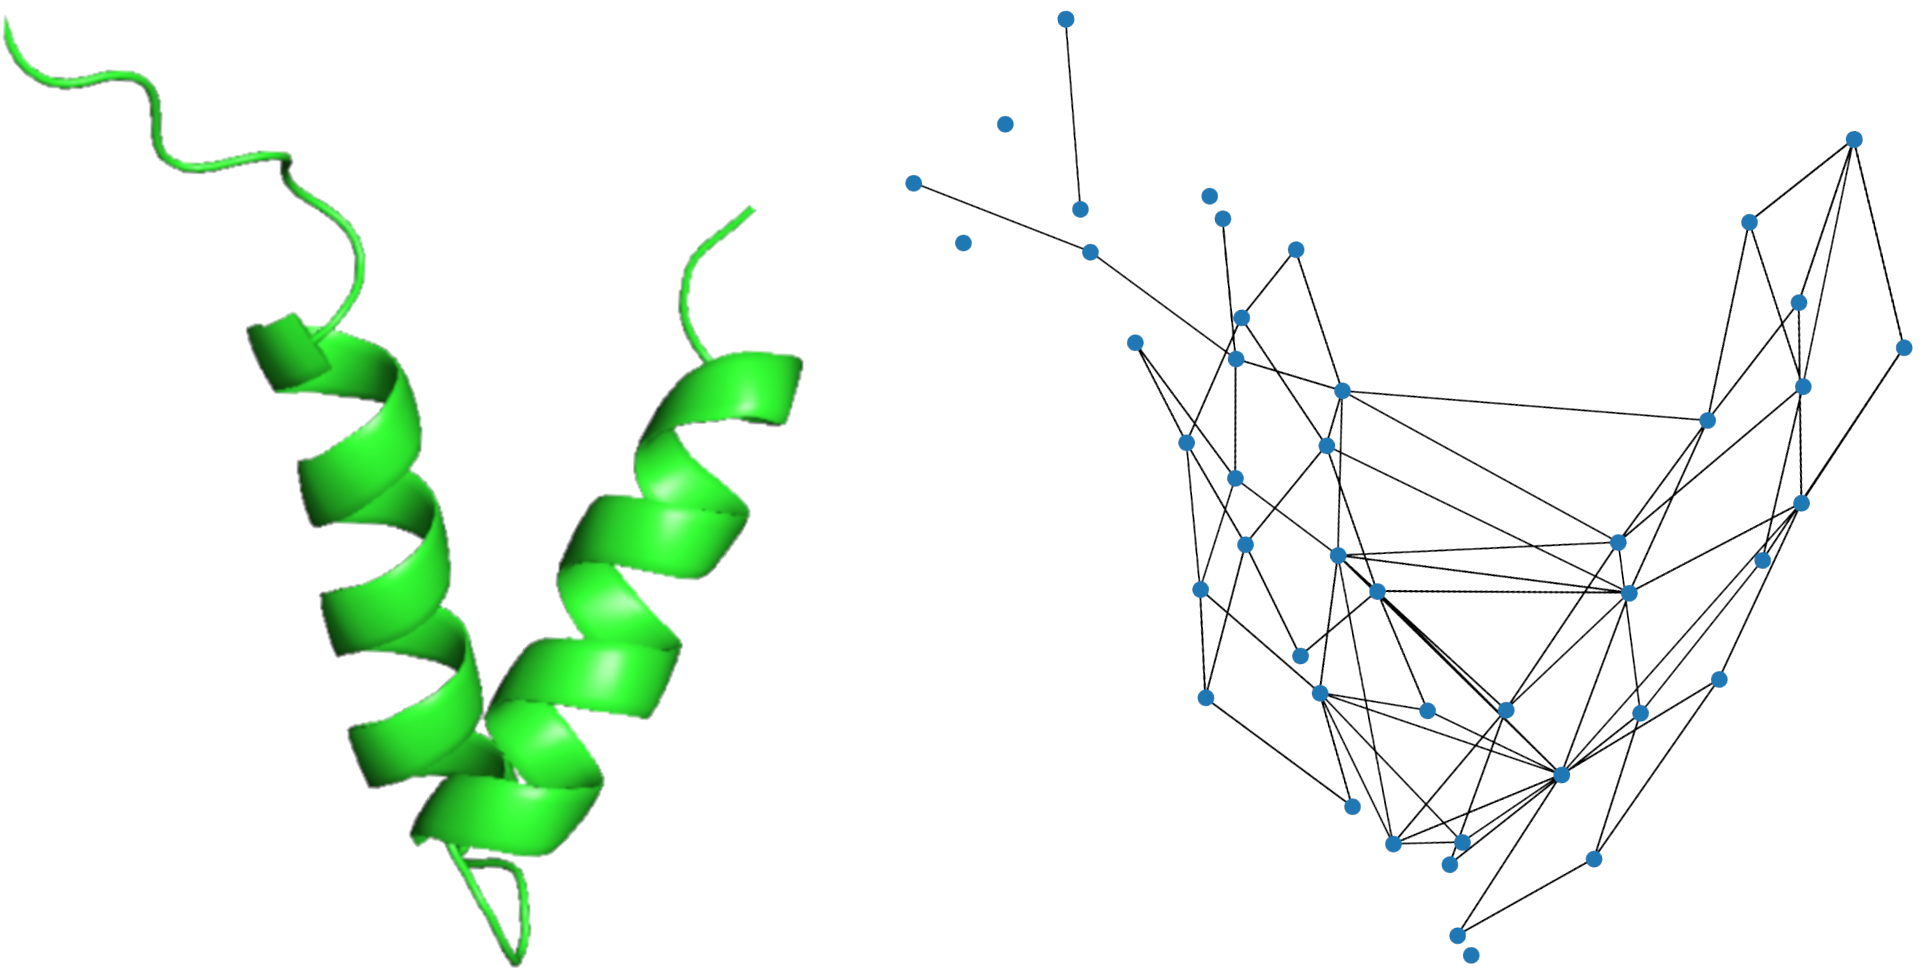
\includegraphics[width=0.5\textwidth]{fig/chain_to_RIN.png}
    \caption{The standard amino acid residues, groupped by properties.}
    \label{fig:AA-prop}
\end{figure}


Secondary Structure\\
Secondary structure of a protein refers to the most common local conformal patterns observed in the polypeptide chains constituting proteins. These patterns promote hydrogen bonding between atoms in the back bone of residues creating the beginnings of a structural scaffold.
The most common of these patterns are $\alpha$-helicies and $\beta$-strands. 
$\alpha$-helicies are right-handed spirals stabalized by hydrogen bonds formed between the oxygen of a carboxyl group and the hydrogen of an amide of another residue.

$\beta$-strands are linear chains of typically 5 to 10 amino acids. 
steatched out
alternating side chain orientation

$\beta$ sheets
can either be parallel or anit-parallel.
parallel slightly less stable
\begin{figure}[ht] % replace with [H} if position is causing problems.
    \centering
    %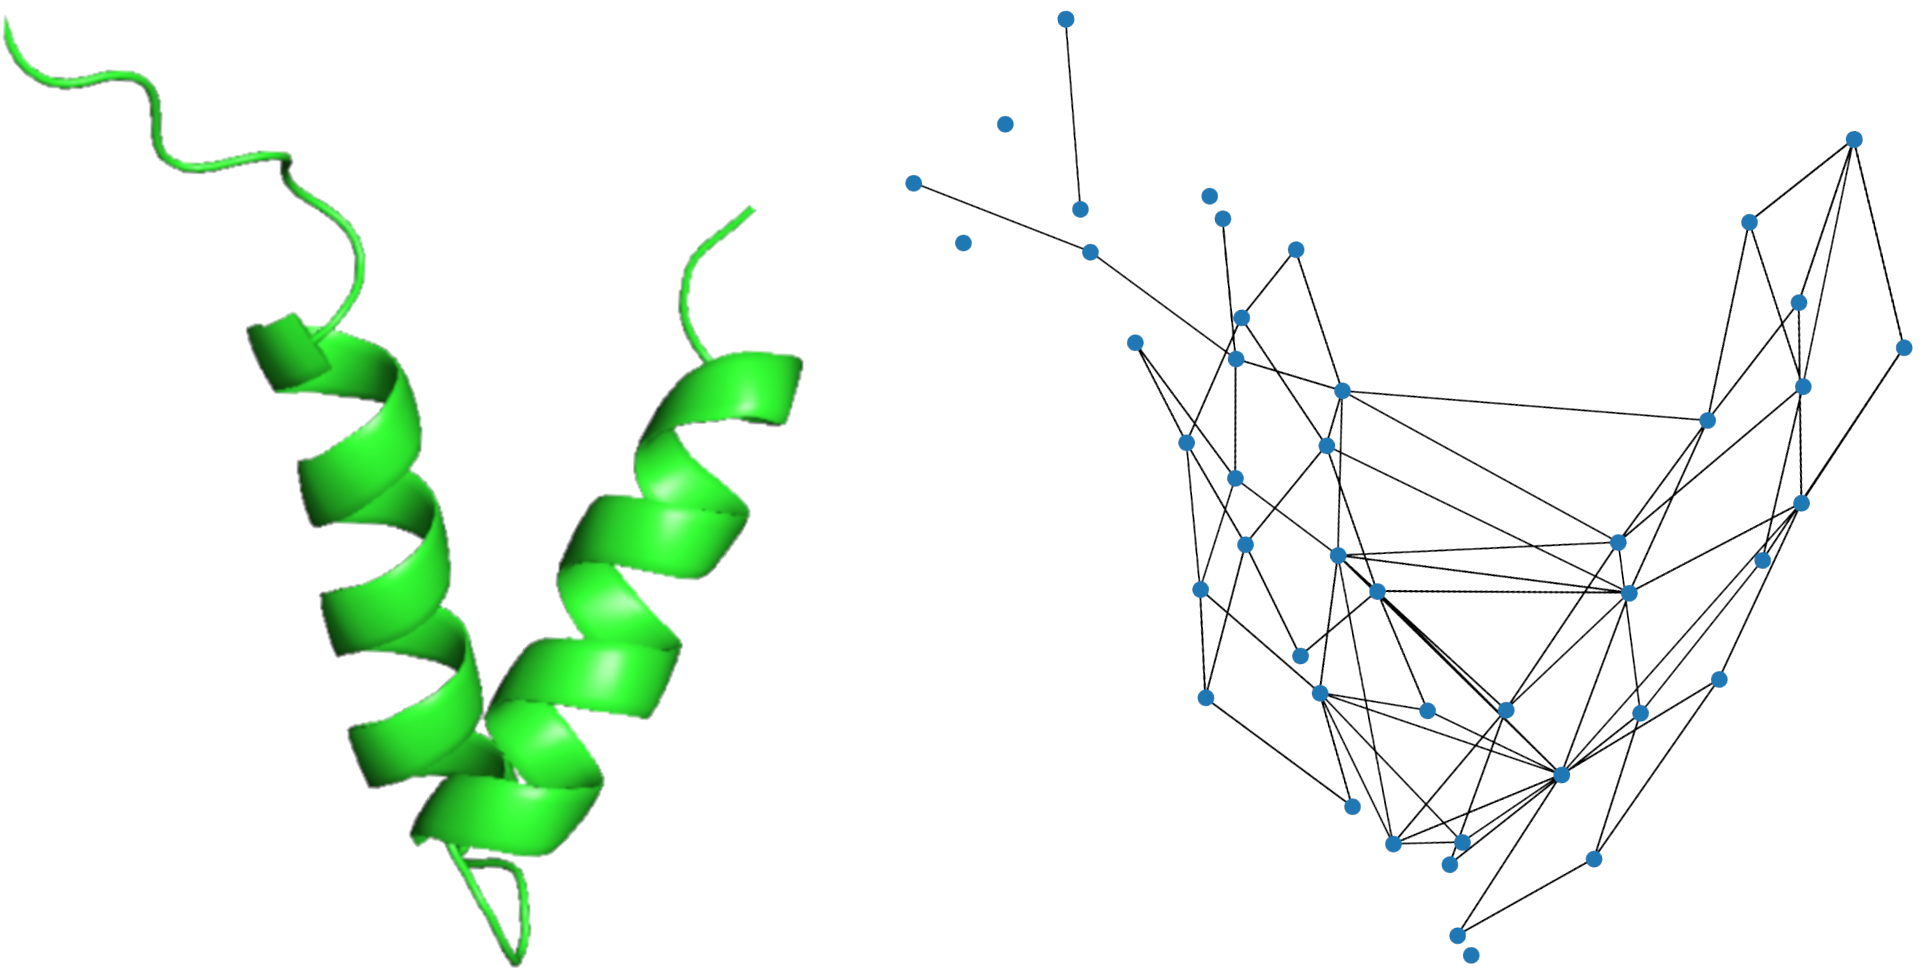
\includegraphics[width=0.5\textwidth]{fig/chain_to_RIN.png}
    \caption{The standard amino acid residues, groupped by properties.}
    \label{fig:secondary-struct}
\end{figure}

Tertiary Structure \& Protein folding\\
Tertiary structure refers to the oerall three dimensional conformation a protein adaps as it folds. This folding is dirven by a process influenced by the cellular enviroment and interactions between the different side chains of amino acids in the polypeptide sequence.
Quatrary Structure \& and protein complexes\\
Quatrary structure refers to the interaction between different polypeptide and other non peptide conpounds, or ligands to create protein complexes. 
These complexes 
It may be the case that a protein chain may occur in only one complex, where as some proteins may have a large network of interactiors with which it is observed in complex with.
We often refer to the spesificity of such interactions to describe the popensity of a protein to bind with only particular partners.

Complexes of multiple proteins are fromed primarially after a protein has folded and are they result of interactions between residues across the different protein chains.
To facilitate partner binding, proteins will have binding substrates with motifs, or notable amino acid sub-sequences, to facilitate a particular interaction. 
These regions or motifs are often critically important to the function of the structure 

Protein structure - function relationship
The final stucture or conformation of a protein is intrensiclly linked to the function of a protein.

\subsection{Homology}
It should be understood how several organisims may be evolutionarly related; from one common ancestor, mutuations are accumulated that may affect an individuals fitness, or the ability to thrive for a given enviroment.
These mutations are often neurtral, having not have much if any obsevable effect; however, mutations that alter fitness are most likely to be negatvie, but some mutations may confer a slight benifit to the individual and become selected. 
Accumulation of these mutations in a sub-population can lead to notably different traits and eventually speatiation. 
The discussion of these evolutionary relationships are well-defined at the orgranism level, but also do much to abstract away the low level on which changes occur. 
At the molecular level, proteins evolve through small changes that may lead to functional variations or the formation of evolutionarily related protein families. Mutations in the DNA of a gene can alter the protein sequence, while structural mutations like insertions, deletions, and inversions may lead to more significant changes. 
This process, known as \emph{molecular evolution}, descibes several different ways in which different protiens may be related. 

Homology is a general term that simply indicates that two or more proteis are related through a common protein ancestor. % find better word then member
%Orthologs
The common ancestor may be quite distant, even occuring befror a speciation event resulting to homologs in different species called \emph{orthologs}. These genes and the proteins for which they code often serve similar functions in the different species.
%paralogs
\emph{Paralogs} are genes within the same species that arise from duplication events of a sigle ancestral gene and result in, initially, two copies of gene and their protein product within the same species. They may diverge over time to adapt different structure or function, but often retain similar ones. Paralogs allow for diversity of similar proteins within a similar species and permit specilization in function.

Homologous proteins are often observed to functional and structural similarities, as mutations that radically impact the function of a protein are unlikely to confer an advantage. 
The theory of homology is frequently used to classifiy proteins into groups or faimilies usiving several different methods to form a taxonomy. 
%Could talk about pfam or cath if you want



Record providing direct evidence for two proteins being homologs most often cannot be established. Instead, homology is typically inferred through similarity between sequences. 
A common task is to find set or family of sequences related to a given query sequence through a \emph{homology search}. 
One such tool for performing these searches is BLAST, or Basic Local Alignment Search Tool, which identifies regions of high similarity between the given query and other known sequences. 
The match is visualize trough a pairwise alignment provided for each pair of query sequence - subject sequence match returned. 
There may be millions of sequences of a database, and inferring homology through a pairwise alignment can be a very difficult and computationally intensive problem. BLAST utility and prolific use can largely be attributed to its efficient implementation of its search algorithm, allowing for fast and accurate set of homologs using a heuristic search method. 
Details about different databases available for homology search and their content, as it pertains to this paper, is discussed in Section \ref{sec:DB-survey}.
% Why study homology

\subsection{Multiple Sequence Alignments}
Multiple Sequence Alignments (MSAs) function to align residues in a set of sequences. These could be sequences of arbitrary symbols. However, MSAs see extensive application aligning sequences of nucleotide sequences such as DNA or RNA, and protein sequences.
% I do not want to explain this
Nucleotide sequences use alphabets of A, T / U, C, G as stand-ins for nucleotide residues --- In DNA, these are adenine, guanine, cytosine, and thymine, respectively. Where in RNA sequences the same residues are observed with the exception of Uricil, denoted with a U, is seen where Thymine is not observed.
 % Protein residues and alphabet should be introduced in a previous subsection
 Amino acids in a protein sequence are identified in this context with a single letter code to designate each residue, as given in Figure~\ref{fig:AA-prop}.
There are many different tools for creating MSAs but all generally work by inserting gaps, designated by a `-', into the sequence. 
Creation of a MSA on a set of sequences typically assumes some form of homology, or evolutionary relationship between sequences in the set. 
A consequence of this assumption is that evolutionarly related sequences will exhibit some degree of similarity.
The use of MSAs allows for examine conserved sites or motifs in a family of sequences. When dealing with protein sequences, these conserved features often correspond to structurally or functionally important aspects of a protein.

\subsection{Structure Files}
%%% 3D structure files aid in the study of the 
The ability to resolve the structure of biomolucules has been transformative to biology as a whole---giving invaluable insigths to the functioning of processes on molecular level. Structural information is now a core aspect in a wide range of fields, providing a deeper understanding of molecular mechanisms that underpin life, from cellular processes to the development of novel therapeutics in areas such as medicine, biochemistry, and biotechnology.

%%% Experimental methods
Protein strctures are determined experimentally using methods such as X-ray chrystallography, nuclear magnetic resinance (NMR) spectroscopy, or cryo-electron microscopy (cryo-EM). 
X-ray chrystallography requires a purifed protein sample to be chrystallized. Passing a high-power X-ray beam through the chrystal results in the creation of a diffraction pattern that is used to determine the 3-D structure of a protein through numerical methods like inverse Fourier Transform. This results in high quality position information, with enough spacial resolution to accurately determine the position of individual moldecules. The need for a high purity chrystal sample, however, can pose a significant limitation, as proteins with dynamic conformation such as intrensically disordered proteins (IDP), or highly hydrophobic proteins like trans-membrane proteins (TMP) can be difficult to chrystallize, resulting in bias in the structural information avaible using this method \cite{PDB-bias}. \todo{An image could be inserted here if filler is needed.}
%MNR
NMR explotis the magnetic properties of atoms nuclei to resolve their position. NMR works by applying a magnetic field to a protein sample and detecting the energy released as the atomic nuclei return to their original states, which helps determine the distances between atoms. NMR has the benifit of being able to study proteins in solution, allowing for observation in conditions that may more similarly resemble their normal biological conditions. Furthermore, the technique is particularly useful for observing the conformal dynamics of flexiable proteins. 
%Cyro-EM
Cryo-EM involves rapidly freezing protein samples in a thin layer of ice to preserve their native structure, then using  electron microscopy to capture high-resolution images of the sample. Thousands of these 2D images are collected and combined using computational techniques to reconstruct a 3D model of the protein. This method is particularly effective for studying large molecular complexes and proteins that are difficult to crystallize.

% Alpahafold aside
Accessiability to strucutural information obrained by such experiments has been revolutionary for the feild of Bioinformatics. This is facilitated by standardized file formats for structural data and databases to catalogue and facilitate access to information. The Protein Databank (PDB) is the foremost database for structural data, offering a comprehensive resource for published experimental structures. 
% more about the database
The avaibility of experimental structural data enabled the training of models such as RosettaFold and Alphafold, which are both machine learning models capable of creating high accuracy predictions of protein structure given an amino acid sequence. Predictions for AlphaFold2 are catalogued in a database and publically avaible. More information about AlphaFold and its structure database are avaible in.\todo{link ref}

As previously mentioned, strucute files availible in such databases are stabdarduzed to aid in machine and human readability. One of the notable early efforts to do this was with the PDB file format, wich still enjoys prevelence, but is in the process of being displaced by the more recent PDBx/mmCIF format (eXtended PDB/Macromolecular Crystallographic Information File). In this work we focus on the mmCIF file format, commonly refered to as just CIF, as HomologyRing is made to work exclusively with this file format.
%%% Introduce CIF, give schema and data higharchy.
The CIF format uses dictionary-based schema allowing for notable extensibility, allowing for effective storage of many different data types. 
A great deal of metadata are included in these structure files; giving biological context to the structure by giving experimental and author information, indicating what genes and organisim a protein chain was transcribed from, pH information and other physical information, what experimental methods were used, mutation information, amoung others. 

%%% Organization of CIFs
Perhaps the most important section of a CIF details the position and identity of atoms in the structure. This is detailed, internally, in the \texttt{\_atom\_site} category, and adhears to a heigharical structure wich is important for the both the biological asseblies of protein complexes and working with said structures in a structural Bionformatics context. In a CIF protein structure, individual atoms will have a set of identifing and associated information like a numerical identifier, symbol corresponding the atoms element, 3-D coordinates, compositon ID, a sequence ID, and chain identifiers. 
The composition ID, sequence ID, and chain identiefiers are both used to assign atom membership to groups within the CIF data higharchy. This higharchy formalizes biologically relevant concepts used to describe polymers like DNA and proteins into a well-defined data structure with several levels: atom, residue, entity, chian (molecule), and structure (complex). Atoms belong to residues in polymers. In proteins these are the individual peptides which are identified within the \texttt{\_atom\_site} section of a CIF by their composition id with their abbreviations like `ALA' for Alinine, `CYS' for Cystine, or `PRO' for Proline, for example, with a similar system for the nucleic acids. Residues are assigned a numerical index, or sequence ID, with in their polymer chain

Additionally, some atoms not belong to the a macromolecule -- polymers like RNA, DNA, or proteins which are most frequently the primary subjects of study in CIFs. such atoms are reffered to as `hetroganous atoms' or \texttt{HETATM} for short. These capture metal ions, water molecules, or ligands, that are biologically relevant to and captured along side the experimental structure. Ligands are molecules that bind to a larger molecule to form a complex and play essential roles in biological processes.

%%% TODO 10/31
% Finish explaing residues, chains, and entities
% reference image
% integrate already written content
% mess around with centrality

\begin{figure}[ht] % replace with [H} if position is causing problems.
    \centering
    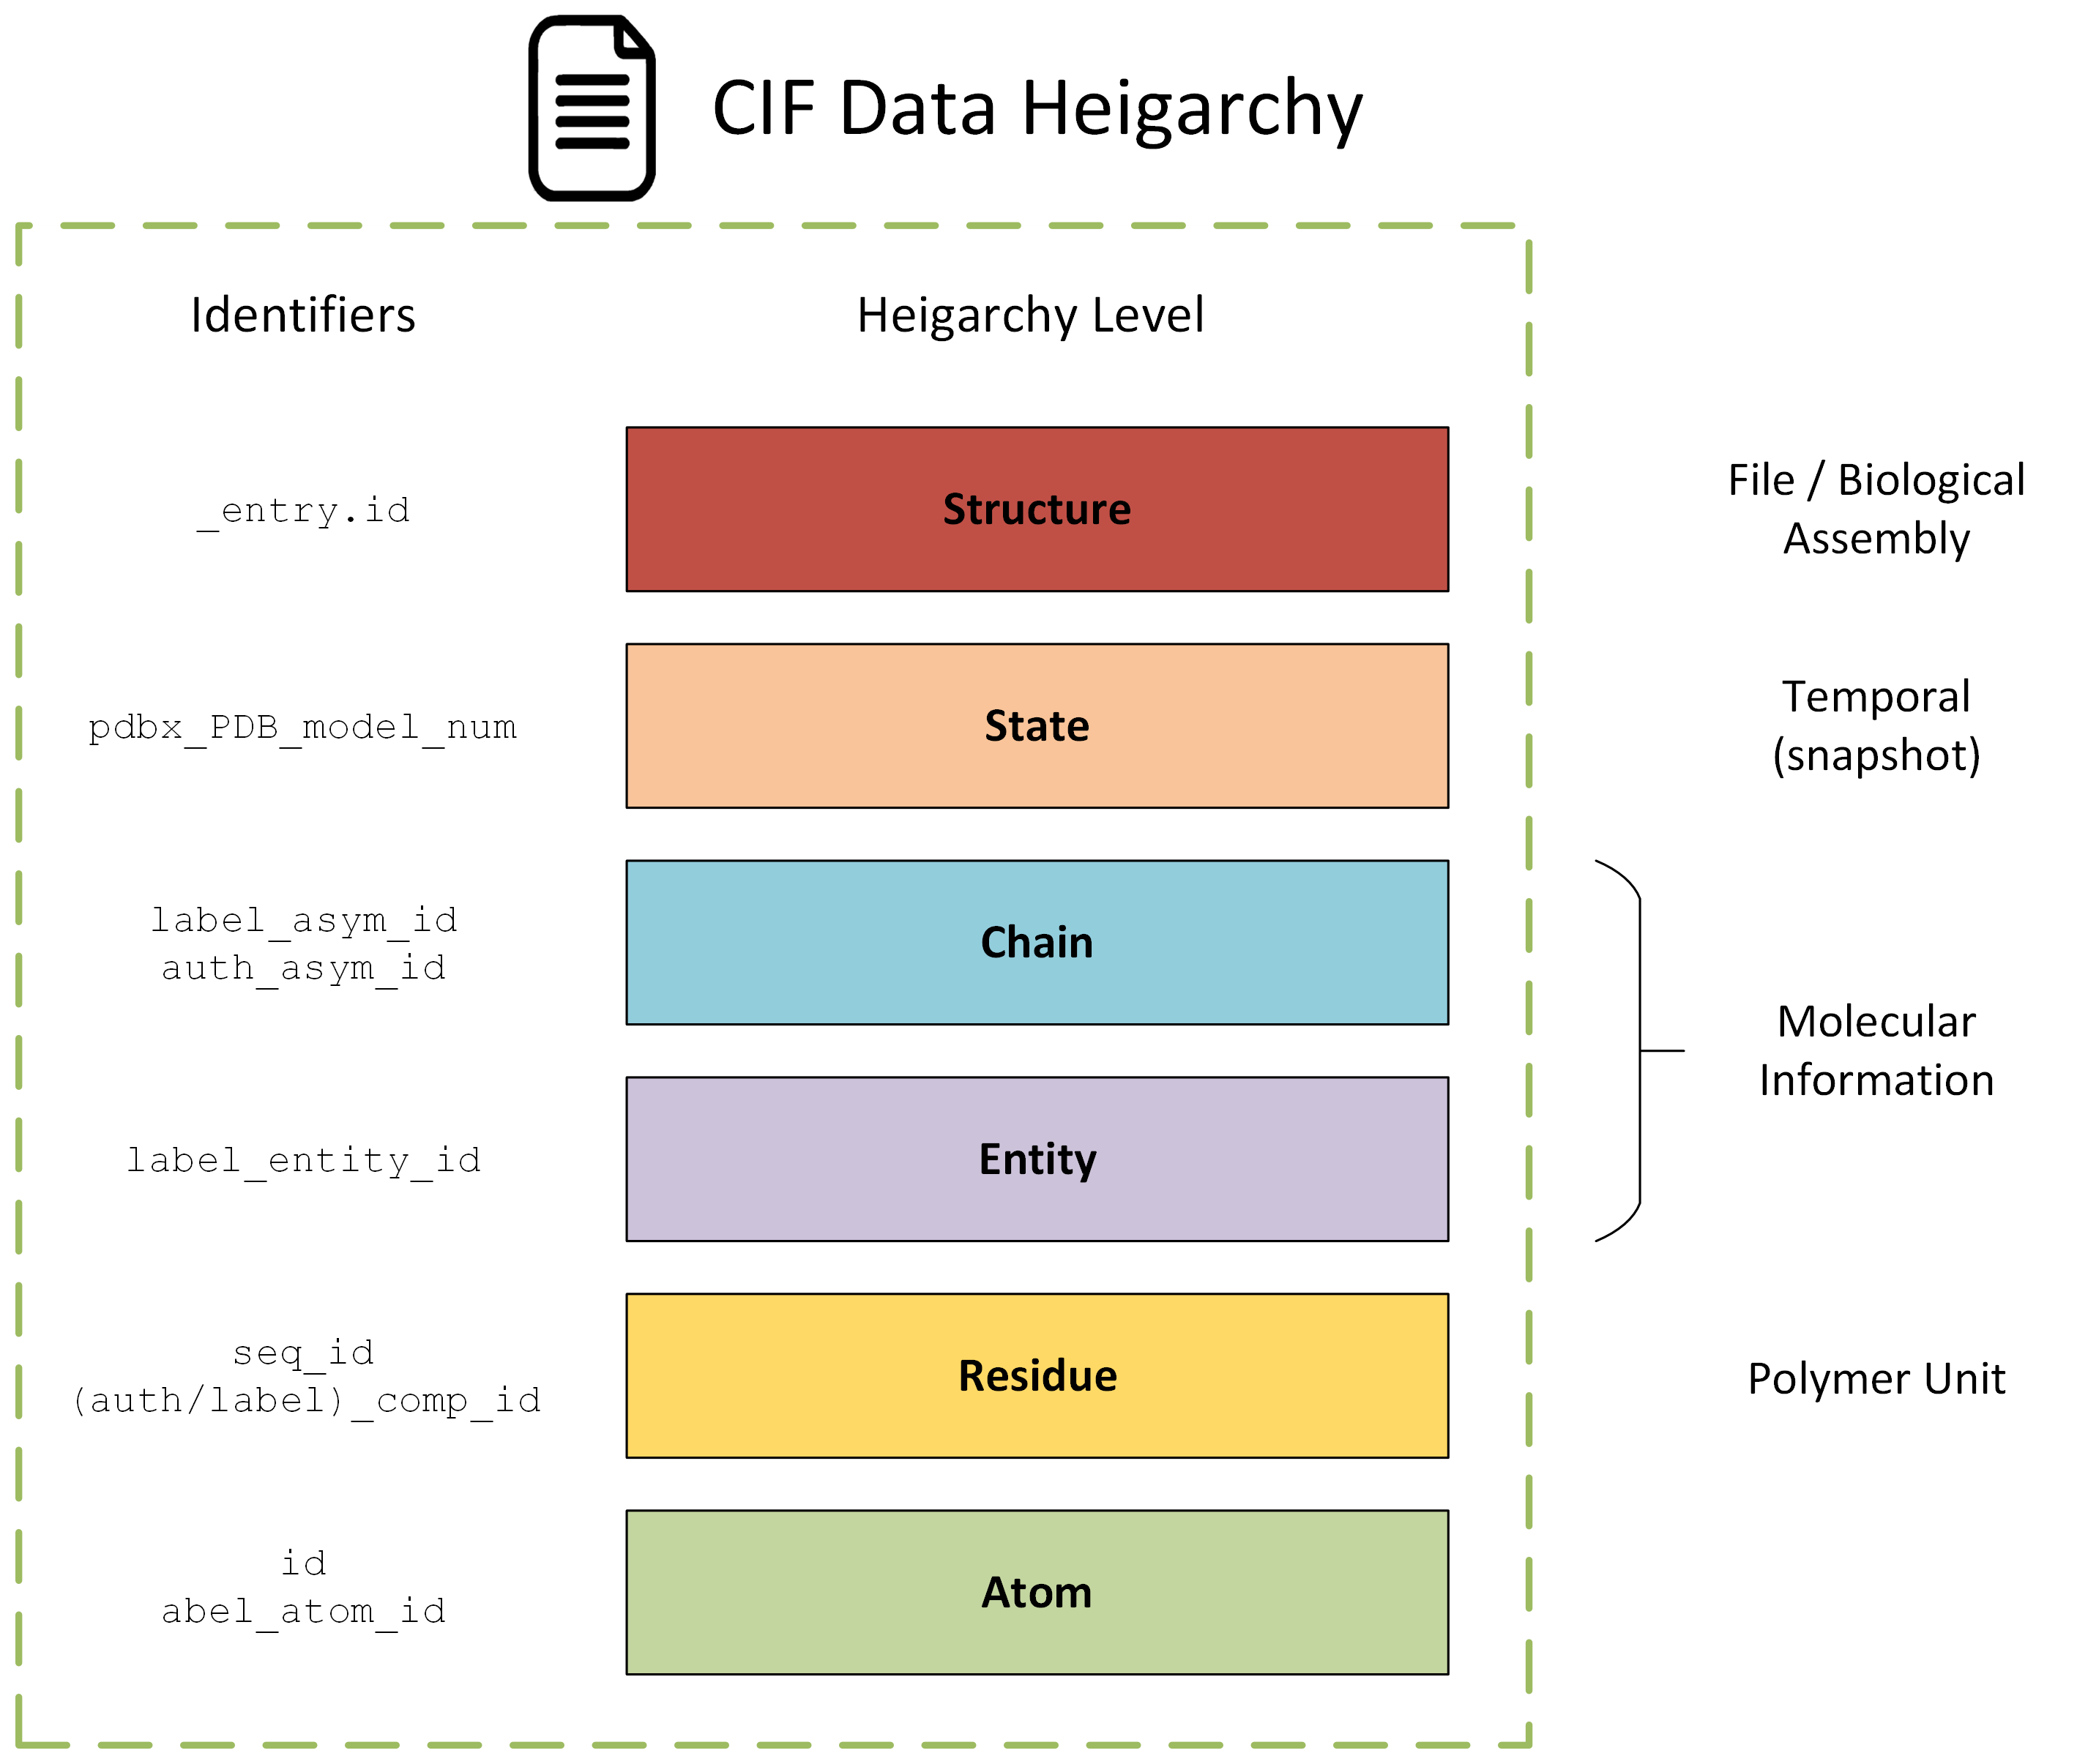
\includegraphics[width=0.5\textwidth]{fig/CIF_data_schema.png}
    \caption{Diagram displaying the various levels of the data organization of structural information in the CIF format.}
    \label{fig:CIF-heigharcy}
\end{figure}

CIFs are supported by a host of software common for structural analysis. Structural viewers like PyMol and Chimera  allow for visual interpretation of a structure which is immediately quite useful for gaining an intuition for the conformation of a protein. However, this is still not without limitations: structuers are often large and quite intricate, requiring the use of cartoon representations of chains to limit the amount of visual information presented to a user. Furthermore, intrepiting functional consequence of strucutres often take a lot of time and biological expertiese. This problem is aided by anotations present in structure databases, as well as many different software tools for performing spesific analysis such structures, something we do as well in this work. % bad wording
HomologyRing supports the use of either PDB or AlphaFold Database for homology search. The choice of which to use will depend on the motivation of their analysis. Differences between these databases and the benifitis of each source is discussed in Section \ref{sec:DB-survey}
.%%% CIF file higharchy
Each structure of a family will contain atleast one entity. These entities may be polymers such as DNA, RNA, or polypeptides; or non-polymer entities like water, or other compounds like co-factors. Each entity is given its own numeric internal identifier within a cif file, which are grouped into chains, identified by a character code. 
%%% Blurb on why HomologyRing is based
Structure files of this form can be quite large, commonly 10s of megabytes, and repositories of structures rapidly become very large.
The PDB contains on the order of 300 GB of structural data and the AlphaFold Database is estimated to be between 20--30 TB. 
This makes performaing analysis at scale of such files, as needed for homology studies potentially quite storage intensive.

The CIF format does has the benefit of being both human readable in text form and machine parceable. However, information about the geometry of the structure is given by the position of discrete atoms. This makes extracting biologically relevant information that one may want from 
Both of these factors can make inferring relevant information from structures at scale quite difficult. HomolgyRing provides a method for encoding structural information for a family of proteins into a network. The process of which is outlined in Section \ref{sec:hRIN}.

\section{Residue Interaction Networks}
At the very basic level, protein chains are polymers of amino acid residues bound together by covalent bonds. As a chain folds, it is \emph{non-covalent} interactions between residues that are principally responsible for the secondary and tertiary structure (conformation) of the protein. These non-covalent interactions could be a verity of different forces and are the result of the different chemical and physical properties of the 20 different base amino acids and their arrangement in the peptide sequence that constitutes the protein chain. 
Examples of interactions commonly observed witnin proteins include Van Der Walls forces and hydrogen bonding. Other interactions are observed less frequently and exibihit high specificity with respect to amino acid participants, like Ionic bonds or $\pi-\pi$ interactions and several others. 
%Need to mention the structure component again
Furthermore, the structure of a protein is intrensically tied to it's function within its biological context. % Why are you mentioning this here
With this in mind, there's a lot of information that can be gathered from knowledge of these non-covalent interactions. 
Researchers may very easily interpret the structural or functional significance of an interaction, but methods concerning non-covalent interactions can be applied to a problem long troubling structural bioinformatics: The amount of available structural information has been growing at a near exponential rate. % citation
Both experimental structures available through the PDB and high accuracy predictions given by AlphaFold2 are commonly available in PDB or mmCIF file formats. These files are large---containing 3D atom data, chemical information, and a host of metadata. Parsing, and algorithmically extracting functionally relevant information algorithmically proves to be an arduous task in many contexts. 
One approach to addressing this problem has garnered much attention: The construction of Residue Interaction Networks (RIN) use information of non-covalent interactions to create a simplified representation of a protein structure.
There are many variants of the idea. However, they are generally defined for a protein structure to be a mathematical graph, or network, denoted $G = (N, E)$ where $N$ is a set of nodes identifying amino acid residues or various compounds in a structure and $E$ is taken the set of non-covalent interactions observed in the given structure.
An example of such a network is shown in figure \ref{fig:ex-prot-RIN}. RINs can be seen to provide a simplified means of capturing the topology of a protein structure, and has seen notable attention for its various applications:
%Applications of RIN
Binding, protein engineering... 
Training data of machine learning methods like graph neural networks (GNN). 
Historical methods like Convolutional neural networks (CNN) on distance matricies discard physicochemical information and may be considerable larger than analogous representation of the same structure with a RIN. 

\begin{figure}[ht] % replace with [H} if position is causing problems.
    \centering
    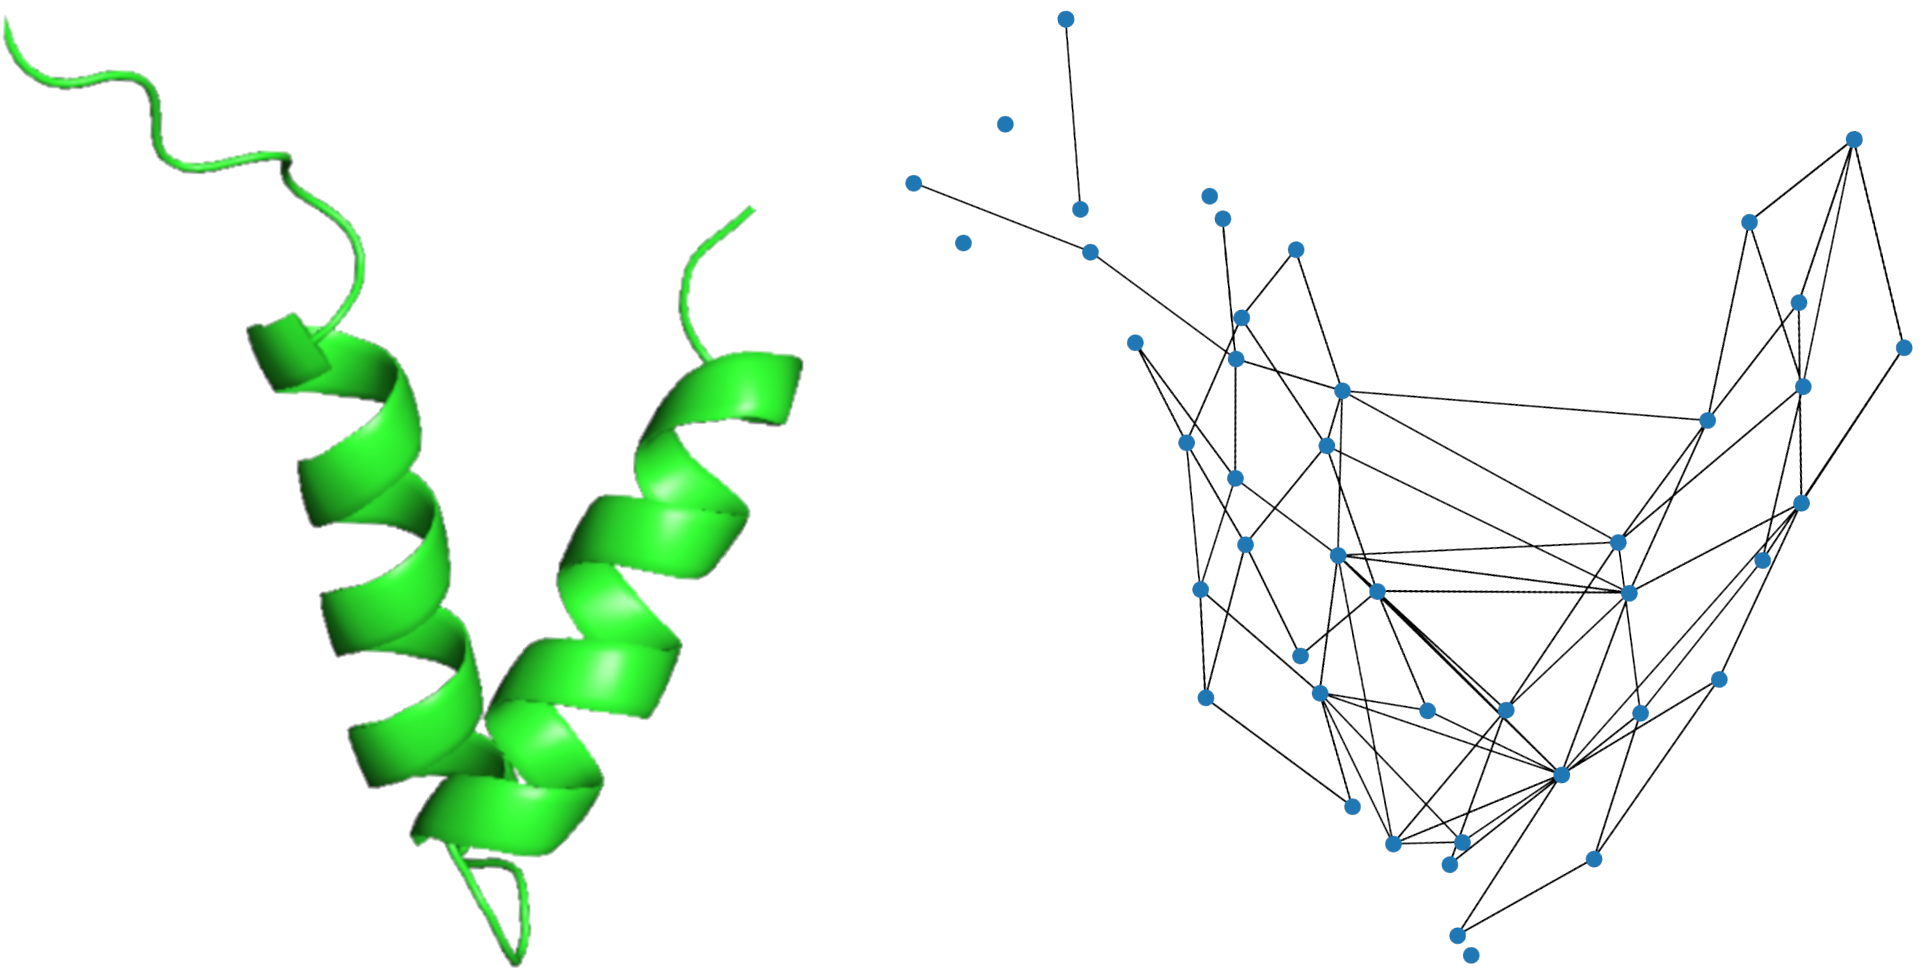
\includegraphics[width=0.5\textwidth]{fig/chain_to_RIN.png}
    \caption{Example of a basic RIN for generated for a protein chain.}
    \label{fig:ex-prot-RIN}
\end{figure}

\todo{If you are going to weight edges with prob for ensembles, it should go here.}

\subsection{Residue Interaction Network Generator - RING}
There are many available tools capable of generating RINs, each with a slightly different interpretation of the object. In this work, such networks are created using Residue Interaction Network Generator - RING. Notable for its ability to handle all ligands and modified residues in the PDB, it is regarded for accurately and deterministically predicting non-covalent interactions within structure files. It is worth noting that the output of RING is a multi-Graph. Differing from the typical mathematical notion of a graph, it permits multiple edges between a given pair of nodes (see Figure \ref{fig:ex-RING}). These different edges correspond to the different non-covalent interactions predicted by RING. The list of interactions predicted by RING comprising the possible edge types in the resulting RINs are described in Appendix \ref{appendix:RING-inter}. Furthermore, we will refer to the various interaction types by their internal RING identifiers throughout this text for the sake of brevity and clarity (e.g. \texttt{HBOND} for hydrogen bonding and \texttt{IONIC} for salt bridges).

\begin{figure}[ht] % replace with [H} if position is causing problems.
    \centering
    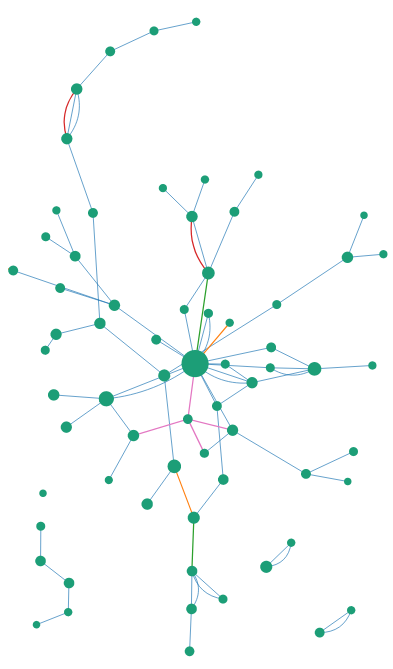
\includegraphics[angle=90, width=0.5\textwidth, height=0.3\textheight, keepaspectratio]{fig/ex_RING.png}
    \caption{Example of a RIN multi-graph visualization created with RING. As typical with RINs, nodes correspond to amino acid residues in a given protein structure. Edges correspond are non-peptide interactions or bonds between residues. Where edges of many interactions are types are permitted between a pair of nodes.}
    \label{fig:ex-RING}
\end{figure}

\section{Appendix: RING - Predicted Interactions} 
\label{appendix:RING-inter}
RING predicts and classifies various types of molecular interactions based on deterministic factors such as geometric orientation, distance, and the chemical nature of the compounds involved. These interactions differ significantly in their chemical and physical properties, including strength and specificity, which in turn influence the likelihood of different amino acids forming specific bonds. Understanding these variations is essential for interpreting the structural consequences and functional roles of these interactions on the atomic and protein level as well as in the context of RINs and hRINs. This section will define and provide context for all interaction types classified by RING, enabling a better understanding of their role in protein structure and function.

\subsection{Van Der Waals Forces - \texttt{VDW}}
Van der Waals forces are relatively weak non-covalent interactions between molecules or atoms. In fact, they they are considered one of the weakest interactions observed at the atomic level. 
VDW forces arise from temporary shifts in electron density induced by the proximity of other molecules or atoms. These shifts occur because of fluctuations in the electron cloud, leading to temporary dipoles. As a result, Van der Waals forces can be either attractive or repulsive.
At very small distances, the repulsive forces dominate due to the proximity of electron clouds, while at larger distances, the attractive forces generated by induced dipoles become prominent. This balance creates a stable equilibrium distance, which plays a key role in maintaining weak but widespread interactions.
%With this in mind, there are three different types of Van Der Waals forces: \todo{I don't think most biologists/users care}
%\begin{itemize} 
%	\item \textbf{London Dispersion Forces}: 
%	\item \textbf{Dipole-Dipole Interactions}: 
%	\item \textbf{Dipole--Induced Dipole interaction}
%\end{itemize}

In proteins, the have prolific presence, as they arise from virtually all residues that would would considered to be in contact. Though individually, a VDW interaction represents a small force, their accumulative effect over large substrates allows them to play a significant role in tertiary and quatrnary structure. 
They are of notable interpretation in the context of RINs, where a great of protein topology is captured by VDW forces, as they can be used as an indicator of residue proximity. However, in practice, they often prove difficult to use in this way. Working with structure or topology information directly can be a complex task. Furthermore, they provide a great deal of data, with a residue often experiencing VDW interactions with many other residues. This surplus of data often hinders the extraction of useful information. 
In a protein family, the VDW interactions tend to be poorly conserved, and given their abundance, it is difficult to prescribe functional importance to a subset of VDW interactions in a family. For this reason, we often choose to filter them in our analysis to highlight the effect of more interactions with higher specificity.

\subsection{Hydrogen Bonds - \texttt{HBOND}}
Hydrogen bonds are most prolific non-covalent interactions second to VDW forces. They are most commonly observed 
in their role of maintaining secondary structure components: $\alpha$-helices and $\beta$-sheets. 
Hydrogen bonding is most prevalent in amino acids with polar side chains, where electronegative atoms like oxygen, nitrogen, and sulfur

However, they are also commonly observed among tertiary interactions, stabilizing the overall conformation of a chain, and quaternary interactions to form complexes. Hydrogen bonding is additionally of notable importance for protein-nucleotide interactions \cite{}. 
Residues most commonly forming these interactions are serine, threonine, asparagine, and glutamine. \cite{}

Information of hydrogen bonding in protein families provides is quite useful, despite their prolific nature. 
it is commonly observed that the preservation of local conformation of functional sites will be critical, even in a family of distantly related proteins. Conservation of hydrogen bonding corresponds to regions of high sequences conservation for interactions of short distance
\subsection{Ionic Bonds - \texttt{IONIC}}
Ionic bonds occur at the atomic level when an electron is transferred from one atom to another. The resulting atoms, having transferred an electron, become ionized hand have and each have a net charge. The donor will exhibit a positive charge, while the recipient becomes negatively charged. This difference in charge, creats a strong electrostatic attraction, bonding the two atoms. 
In proteins, ionic bonds are often referred to as \emph{salt bridges}, and their formation generally require the presence of amino acids with charged side chains. These include: lysine, arginine, and histidine with positive charge; and asperic and glutamic acid have negatively charged side chains.
This creates a loose relationship between conservation of these residues in a sequence and the conservation of ionic bonds they may participate in in a structure. % Possibly remove. At very least reword.
The ability of the charged amino acids to participate in ionic bonds is pH dependent. This allows some proteins to adapt variable conformations in response to cellular environment; this is one possible functional interpretation of an ionic bond with in a protein.

\subsection{$\pi-\pi$ Stacking - \texttt{PIPISTACK}}
$\pi$-$\pi$ stacks are spesifc interactions between pairs of aromatic rings; or stable, planar, ring-shaped molecular structures with alternating single and double bonds present in some amino acid side chains.
In proteins, such amino acids with requierd for the interaction are: phenylalanine, tyrosine, histidine, and tryptophan. 
These aromatic rings have decentralized $\pi$-electrons, to which the interaction owes its name. 
These electrons have distributions not centralized around a single atom, as typically the case, but rather the electrons may exist in a shared annular cloud around the aromatic ring.
These perculiar electron distributions permit specialized interactions: either with other aromatic rings to form a $\pi-\pi$ interactions, or other compounds, as seen later.

$\pi-\pi$ interactions may have one of two possible configurations of the participating aromatic rings: 
\begin{itemize}
    \item \textbf{Face-to-face}: where the rings are stacked directly on top of each other with a slight offset.
    \item \textbf{Edge-to-face}: where the rings are oriented perpendicularly, with the edge of one ring pointing toward the center of the other.
\end{itemize}
In both cases, the interaction of the $\pi$-systems creates an attractive force that stabilizes the residues relative positions.

These interactions tend to be quite specific and relatively well preserved.
Often serve to stabilize tertiary and quatrary structure. Given this role they are quite useful for characterizing a families topology.

\subsection{$\pi$-cation Bond - \texttt{PICATION}} \todo{both pi cation and pi pi stacking have noteworthy roles in binding with pi systems in ligands}
Similar to $\pi$-$\pi$ interactions, $\pi$-cation interactions require the particular electron distribution of a $\pi$ system seen in an aromatic ring. However,

Donor cations can belong to another residue with a positively charged side chain, allowing the interaction to play a notable role in tertiary and quatrary structure stabalization.
Beyond intra or inter--chain interactions, $\pi$-cation interactions or often important for ligand binding and in enzyme active sites; where aromatic residues can be used to locate cations and stabalize interactions.

in these interactions the system is to considered to donate a $\pi$ electron to the cation, which becomes a $\pi$-acceptor.

\subsection{$\pi$-hydrogen Bond - \texttt{PIHBOND}}
Similar in action to both $\pi$-cation bonds and typical hydrogen bonding, $\pi$-hydrogen bonds are stabalizng interactions where a positively charge hydrogen bond donor, such as a polar \ce{-OH} or \ce{-NH} group, interacts with the electron rich $\pi$ system of an aromatic rings, present if several amino acid side chains.
$\pi$ hydrogen bonds are weaker and far less common than both $\pi$-cation and $\pi$-$\pi$ stack interactions. As a result they tend be less frequently important for the structure and function of a protein, and they are observed to often not constitue a significant part or residue interaction networks. However, there are notable exampels where they perform a significant role, such as in DNA binding proteins such as transcription factors and aromatic rich enzyme active sites. \todo{this is interesting. see if you can expand on the DNA binding}

\subsection{Halogen Bonds - \texttt{HALOGEN}}
Halogen bonding is a non-covalent interaction involving a halogen atom (such as fluorine, chlorine, bromine, or iodine) and an electron-rich atom or group (such as oxygen, nitrogen, or sulfur) acting as an electron donor. Although halogens are typically considered electronegative, when they participate in covalent bonds, they exhibit a region of positive electrostatic potential called the $\sigma$-hole on the side opposite to the bond. This $\sigma$-hole allows the halogen to act as an electron acceptor, facilitating the formation of a halogen bond with an electron donor. 
In proteins, 

\subsection{Disulphide Bonds - \texttt{SSBOND}}
Disulphide bonds, also called disulphide bridges, are uniqe in this list of interactions as they are covalent bonds; and the amino acid cystine is also unique for its sulpfur containing \ce{-SH} thiol group in its side chain, need for the formation of disulfide bonds.
The formation of the sulfur bridge reqires an oxidation reaction where the hydrogen is displaced, and results in a \ce{S-S} interaction that is considerably stronger and more sable than many of the other inter-residue interactions witin a protien. That said, they are reversable under reducing conditions, allowing for dynamic protein conformations that are responsive to certain cellular conditions. The strength of the covalent bond is durable in harsh extracellular conditions, and is often seen stabilizing structure in such enviroments. 
These bonds are generally seen to have notable separation in a protein chain or present in typically well preserved inter-chain interactions. \todo{cite and more details}
This gives cystine a clear role in contributing to tertiary and quaternary structure of proteins. 
Due to the unique nature of cystine and disulfide bridges, cystines are frequently well preserved at the sequence level within a protein family and so too are associated disulfide interactions.
Cystine is notable for participating in other interactions such as metal coordination, or enzymatic activity, but where it participates in in disulfide bridges, tend to represent highly conserved sites within a protein family.

\subsection{Metal Coordination - \texttt{METAL\_ION}}
Involves the interaction of a metallic cation.
Metal Coordination bonds can be covalent, where they are also called dative bonds, or non-covalent.
Even non-covalent metal coordination interactions tend to be high strength interactions.
Coordinate Covalent bonds are particular because a pair of electrons involved from the bond are donated by a single atom (often nitrogen, oxygen, or sulfur) and paired with an electron-deficient acceptor. 
Since the donor contributes a pair of electrons, the most common acceptors for this type of interaction are \ce{Zn^{2+}}, \ce{Fe^{2+}}, and \ce{Cu^{2+}}.

Metals in proteins have a key roll in electron transfer processes, allowing proteins to facilitate redox reactions. 
Finally, centrally coordinated metals often of great strucural significance, as the strong coordination interactions work to stabalise the conformation of a protein as is the case with zinc finger proteins where cystine and histidine bound to a \ce{Zn^{2+}} ion gives the structure its iconic shape, enabling DNA and RNA binding. 

Metal coordination, then, most often represent critical components of a proteins structure or function and consequently are frequently well perserved in families. However, experimental and procedral variation in structure creation can make there presence inconsistent in some senerios. Notably, AlphaFold2 does not predict the presence of metals, or other ligands, so will not be represented in predicted structures.  

\section{Appendix: Installation and Dependencies}
The code repository can is available from the BiocomputingUP GitHub: \\
\href{https://github.com/BioComputingUP/ring-homology-pipeline}{https://github.com/BioComputingUP/ring-homology-pipeline}\\
Execution of the pipeline has a set of commandline programs be installed and correctly added to \texttt{PATH}. 

\vspace{0.5cm}

\begin{tabular}{l l}
\textbf{BLAST Command Line} & \url{https://www.ncbi.nlm.nih.gov/books/NBK279690/} \\
\textbf{Clustal$\Omega$} & \url{http://www.clustal.org/omega/} \\
\textbf{RING standalone} & \url{https://ring.biocomputingup.it/} \\
\end{tabular}
\vspace{0.5cm}

Note that ring4.0 command line is needed for use of \texttt{use\_label\_asym\_id} argument when building a hRIN. 
Additionally, commandline BLAST requires copies of databases be built and installed locally inorder to perform a homology search. The two that we display in this paper and are likely to be of particular interest to a user is `\texttt{swissprot}' and `\texttt{pdb}' which may be downloaded from the BLAST FTP server. Files, typically in FASTA format must be built into blast databases using the BLAST commandline tool and placed into the \texttt{blast\_db} directory. 
The user may alternatively create their own blast database with the same method, however, it should be noted that the resulting database may have a different schema and the config file: \texttt{config.json} may have to be modified to allow for successful parsing. \todo{Trying to deprecate this, if possible}
Specifying that the homology search should be performed remotely with the \texttt{remote\_BLAST} argument can avoid the need for a local blast installation. However, it should be noted that the search usually takes much longer on NCBI servers.
\section{Methods}

\subsection{Pipeline}
%overview
The tool is implemented as a python package responsible for running the pipeline and conducting supporting analysis. 
The execution of the pipeline to construct a hRIN represents the primary responsibility of the python object and must be ran after object initialization to perform any useful subsequent action on a hRIN. % Would be useful to load hRIN from file.

An overview of the pipeline steps are as follows:
\begin{enumerate}
	\item The pipeline is initiated for a query protein chain identified in a CIF file or a list representing a family of homolog chains is provided by the user.
	\item For a query chain, AA sequence is used as a query for a BLAST homolgy search of either the AlphaFold or PDB database.
	\item Retrieve Structures for homolog proteins.
	\item Multiply align sequences of homolog chains.
	\item Predict non-covalent interactions for each structure with RING.
	\item Synthesize homolog RINs with alignment information to create homology-aware hRIN.
\end{enumerate}


\subsection{Initiation}
The construction of the hRIN is initiated on either a user-chosen query chain or a user supplied family of structure.
In the former situation, the query chain is taken to be a representative example of the protein family - the subject of study that will form the basis of the homolog search and construction of the Interaction network.
To begin, The user supplies a Crystallographic Information File (CIF) that contains the physical information about the query chain. From this file the query polypeptide sequence is extracted and processed to address potential non-standard or unknown residues present in the sequence. Specifically, CIF files will contain a \emph{canonical sequence} for the chain that is the result of some rudimentary processing, simplifying non-standard residues. 
In the ladder case, the pipeline supports analysis of a user defined of protein chains. In this case, the user gives a list of structures which are known a priori to contain homolog chains, forgoing the need for a homolgy search. The user must additionally supply a list identifying which chains withing the structures are the homologs to be considered for the construction of the hRIN (by their internal CIF chain identifiers: label\_asym\_id) in the form of a tsv file containing the name of the structure and the chain ID.

\subsection{Homology Search}
With the query sequence extracted, it is used to perform a homology search with protein-BLAST. The user has the choice to perform this search over either the database of UniProt predictions or the Protein Databank (PDB). 
These database differ in their distribution of contained sequences - with the protein databanks around XXXX protein sequences over XXXX structures representing a notably more biased population than uniprots XXXX protein sequences. 
However, the next step is to automatically download structures for the returned homolog sequences. Metadata describing the map of sequences to their homolog chains in corresponding structures as well as matched regions from the BLAST results are maintained and used for the later construction of the final hRIN.
% Mention BLAST default parameters

\subsection{Structure Retrieval}
%% Not sure if this should go in homolgy search or structure retreival section - it spans both
%% Need the extened information about each database
Due to unreliable experimental structure availability for all of uniprot, choosing to perform the homolog search over the larger database will necessitate that homolog structures be retrieved from the database of AlphaFold2 predictions, which has the notable limitation of contain structures for only a single protein chain. Where searching for sequences over the PDB will result in the pipeline downloading the corresponding experimental structures. These may contain comples of protein chains, other polymers (such as nucleotides) and Ligands. This permits many potential useful analyses. % But has the limitation of...

Once homolog structures are collected, some basic filtering is performed to ensure CIF structures are not malformed, as is sometimes the case in the PDB, preventing the running of RING due to missing secondary structure information, for example. % Information not needed
The peptide sequences of each homolog chain are extracted from the structure. This ensures parody with information contained in the hRIN and the component structures used for its construction, thus avoiding issues caused by out of data BLAST databases and updated PDB/UniProt entries can causing discrepancies. 
Discussion of the different structure databases can be seen in Section \ref{sec:DB-survey}.

In later sections, we regularly refer to a family of structures wich to take to mean the set of structures returned by this process. \todo{finish}

 contains a what we regularly refer to as a \emph{homolog chain} that corresponds to the a sequences identified during the homology search due to its high sequence similarity to the query sequence. In addition to the \emph{homolog chain}, structures in the family, if retrieved from the PDB, are commonly complexes of many entities. It is common that a complex may contain many homolog chains, but we will refer to entities that are not homologous to the query sequence as \emph{non-homolog entities}. These entities are further categorized in Subsection \ref{subsec:node-types}.

\subsection{Sequence Alignement}
% are only blast regions used? - no
% Clustal Omega
The full chain sequences resulting from the operation (not just the sub-sequences returned by BLAST) are aligned into a multiple sequence alignment (MSA) using clustal$\Omega$. This MSA is later used for the identification of nodes within the hRIN.

% MSA figure
Multiple Sequence Alignments function to identify families of corresponding residues in many sequences.
They assume 

\subsection{RING}
Running RING on each homolog structure results in a family of RINs. However, sequence variations across the homolog chains mean that a homology-aware method for synthesizing their information is necessary for the construction of a hRIN. To do this nodes are either defined to be a family of homologous residues or, or a set of non-homolog entities defined across the set of structures. This requires a system of maps relating residues identified in structures as well as indices in BLAST and RING output to columns in the MSA. Non-homolog chain entities are mapped to nodes in the hRIN through a parallel process. The details of node definition are described in Section \ref{sec:hRIN} and Subsection \ref{subsec:node-types}.

\subsection{hRIN Synthesis} % possibly merge into RING subsection.
The final step in the core of the Ring Homology pipeline is the synthesis of the hRIN from previously collected information. The most import aspects of this process include merging homology information from the BLAST search, alignment information from Clustal$\Omega$, and interaction information from RING.




\section{Homology Database}
\label{sec:DB-survey}
% Need to find correct place to discuss AF vs PDB
\subsection{AlphaFold}
AlphaFold is model for predicting the 3D structure of a protein chain given its amino-acid sequence, a challenging and long standing problem in bioinformatatics. AlphaFold2's predictions are renown for their high accuracy, and have proven transformative for the field \cite{alphafold}. 
AlphaFold2 has the notable restriction that predictions are formed for only a single protein chain, not entire complexes of multiple protein chains or ligands - non-polymer structures with which a protein chain is known to bind or interact.  They tend to be of high functional significance, and the subject of many analyses. Ligands are commonly resolved in experimental methods catalogued in the PDB like MNR or X-ray crystallography.
AlphaFold3 predictions include protein complexes and protein-peptide interactions, but have yet to be made widely available for all UniProt sequences via a database.

\subsection{Protein Data Bank (PDB)}
%Inter-chain Contacts
%nucleotide binding

\section{Homology Residue Interaction Network - hRIN}
\label{sec:hRIN}
We use the term Homology Interaction Network (hRIN) to refer to homology enriched RINs.
It should be noted that nodes witin the hRIN do not identify individual residues as they do in typical RINs. Rather, they generally correspond to families of residues as identified by columns in the MSA. In other works this similar concepts of using an MSA to synthasise a set of RINs are called Key Interaction Networks (KINs) \cite{Yehorova2024}. 
\subsection{Contact Conservation}
\label{subsec:def-conservation}
On of the key aspects of homology information encoded to hRINs are edges weighted with the probability or conservation score. This value captures the propensity of an interaction represented by an edge being present in any given member chain of the protein family. 
This required developing different notions of \emph{contact conservation} that can be interchanged depending on the needs of the user. 
The first, more basic, definition simply normalizes the number of observed interactions of a given type for a given pair of nodes by the number of homolog structures in the family. That is, for residue nodes $u,v \in N$ and interaction type $\xi\in\{\texttt{VDW}, \texttt{HBOND}, ...\}$ 
\footnote{The HomologyRing tool supports calculating conservation socres for multiple interaction types at once to support analysis requiring queries selecting multiple interaction types of interest. It only requires that conservation scores also be normalized by the number of selected interactions.} 
(see appendix \ref{appendix:RING-inter}) , we define:
$$p_\xi(u,v) = \frac{1}{|H|} \sum\limits_{x \in H} I_{\xi}(u, v, x)$$ 
where $N$ is the number of homolog structures in the family and $I_\xi$ is simply the indicator function: returning $1$ if nodes $u$ and $v$ are connected by an edge of type $\xi$, else $0$. This does well to normalize interaction counts to probabilities, but has the effect of diminishing some interactions conservation score when it may, in fact, not even be possible in every structure. This is because some nodes may represent families of families of residues given by columns of the MSA with low occupancy, meaning they have gaps or no corresponding residue for some structures. Given the variation seen in the PDB for both indels in sequences, and entities present in complexes, it may be undesirable to penalize such situations for some analyses. To address this, we provide an alternative formulation of conservation:
$$p_\xi(u,v)=\sum\limits_{x\in H}\frac{I_\xi(u,v,x)}{I_\text{non-gap}(u,x) \cdot I_\text{non-gap}(v,x)}$$
\subsection{Inter-Chain \& Ligand Node Identification}
\label{subsec:node-types}
Identifying nodes by families of residues given by columns of the MSA works well for nodes associated with residues in the query structure. However, many structures in the PDB contain a complex of multiple \emph{entities} and many potential analyses performed with RIN concern the interaction of a complex of multiple protein chains and ligands. 
In this context \emph{entity} refers to a structural unit with in structure files. They may be polymer chains (protein or nucleotide) or ligands. \todo{Breifly mention the EIDN system.}
Ligands are small non-polymer molecules, ions or other chemical entities that bind or otherwise interacting with sites of a peptide structure. These can be endogenous molecules like co-factors or signaling molecules.
We make the distinguish primary types of entities for our analysis: protein chains referring and other non-peptide compounds (including nucleotide polymers like DNA and RNA) as ligands. 
With this distinction we classify an edge in a hRIN depending on the entities the nodes the edges connect span. An edge that connects to residues within the same protein chain is referred to as an \emph{intra-chain} edge or interaction. 
Should an edge connect nodes in different protein chains, it is said to \emph{inter-chain}. Finally, an edge connecting a protein chain to a ligand are referred to as \emph{ligand} interactions. 
For the purposes of our analysis we only consider intra-chain contacts to be interactions within chains in the set of homolog proteins, not contacts within chains said proteins may be in contact with. The reasons for this are discussed later in this section.
Furthermore, interactions between non-homolog chains and ligands, and are not included in constructed hRINs. % This choice is not justified by anything other than it would have been annoying to implement. And would be potentially useful for analysis.


When observing the structures within the PDB for a set of homologs it is common to see closely related chains in complex with varying types and quantities of entities across many examples. 
Graphically encoding information of all entities into a homolgy-aware network is challenging. 
There is generally no guarantee that entities present complexes containing a homolog chain in the PDB can be neatly mapped into families across all structures. Given this variability, attempting to encode information about all residues in all present protein in a family of complexes can result in a network that is quite complicated and fails to provide a useful characterization of the family. 

To address this issue we implement a system of identifying corresponding entities across structures returned by the homology search - both protein chains and Ligand compounds. These entities are identified in all structures returned by the homology search. % give a name to this family of structures



With this in mind we can provide a mathematically rigorous definition of the hRIN object that proves useful in later analysis.
In practice, there is much information contained within the nodes of an hRIN, including: 3D position information, consensus residue, residue type.



\section{Analysis Tools}
\subsection{User Defined Queries}
\label{sec:queries}
Given the wide and diverse set of analyses once could potential want to perform on interactions within a protein family, HomologyRing supports users providing a custom query, allowing for the creation and analysis of a sub graph of the initial hRIN created by the pipeline. This sub-hRIN is defined by 3 primary parameters: \texttt{interaction type}, \texttt{interaction class}, and \texttt{region}. 
Filters on \texttt{interaction type} refers to the specific kind of interaction reported by RING. These are listed and described in Appendix \ref{appendix:RING-inter}. This allows users to create a subgraph from a subset of edges of given types.
The different types of non-covalent interactions see different distributions within the PDB. 
Much of the disparity can be attributed to some interactions like \texttt{IONIC} and \texttt{PIPISTACK} may only occur between a specific subset of amino acid residues, but the different interactions are seen to be associated with different structural and functional features. 
RINs constructed from all possible interaction types tend to be quite dense, primarily as a consequence of prolific nature of interactions like \texttt{VDW} and \texttt{HBOND}. The former Van Der Walls interactions are generally present when two neutral compounds are into close proximity and can be either attractive or repulsive. The ladder hydrogen bonds are most commonly responsible for secondary strcture elements within a strcture such as the formation of alpha-helicies or beta-sheets. 
These tend to be generally well perseved within a family of proteins, but can exhibit notabale conservation and variation at binding sites where the homolog chains interface with either another protein chain or a ligand. A protein family that contais many homologs or paralogs that come in complex with a verity of different entities may have a tendency to exhibit interactions spesific to a given entity. where protein chains that are more consistently observed in the same complex will have these sites conserved. % this belongs somewhere else
We later show this to be the case in an example where a famaly of human DDX paralogs are observed to have conserved intra-chain \texttt{HBOND} interactions at binding sites critical for protein function.
Lastly, Hydrogen bonding is also seen to stabalize tertiary and quatary structure to a less common extent. These interact tend to be more variable in families with greater sequence dissimularity. % unsupported, bad asside.
Some of the more novel interactions such as \texttt{SSBOND} are seen to have significant conservation within a family. \todo{move discussion of this to the RING appendix. Be breif here}

Specification of \texttt{interaction class} allows the user to construct a graph out of a subset of edges conditioned on the entities the edges are between. 
Valid choices are intra-chain, inter-chain, chain-ligand contacts, or all and select the respective edges described in Subsection \ref{subsec:node-types}. 
Intra-chain contacts include interactions and corresponding edges between residues in the same protein chain. Consideration of exclusively these edges enable analysis of secondary and tertiary structure variance and conservation within a family.
Inter-chain contacts refer exclusively interactions with participating residues in different protein chains. At a glance, conservation of contacts can deliver insight into which contacts are key to the binding of protein chains to form ligands.
This enables an analysis of binding domains to gain insight into which residues are evolutionary important for interactions or what adaptations in specific sequences may contribute to specificity in partner binding.

Ligands
Metal-coordination can be essential for structure and contain important functional information about a family of proteins.
Co-factors
DNA/RNA

Finally users may place a filter on nodes to be included in the resulting sub-hRIN.
The default behavior is to perform not filtering and include all nodes.
Regions of interest in a family may be specified by the user to create a sub-hRIN that captures interactions with a set of residue nodes. For example, creating a hRIN for an entire structure may provide a lot irrelevant information when performing an analysis on an inter-chain binding substrate conservation within a family. 
Can specify an occupancy ratio, selecting residue-nodes in the network that correspond to MSA columns that contain above a given threshold of non-gaps. This allows users to quickly discard nodes corresponding to the poorly conserved tails of the MSA that are not representative of the family. 
It should be noted that region filters placed on the nodes are not strict, and should an edge have at least one node in the selected region, the edge and both nodes the edge connects will be included in the resulting hRIN.

\subsection{Contat Mask Plots}
\label{sec:contact-masks}
A very quick means of identifying groups of conserved interactions within a family of proteins is the use of \emph{contact mask plots}. These display an image of the MSA used to define the residue nodes in the hRIN. Intuition about the characteristics of each family may be gained by the use of CLUSTAL colors which encodes physio-chemical properties of different residues into color. On top of this is a binary mask indicating that the residue in a given structure and residue family participate in an interaction that matches the users query.



\subsection{Contact Conservation Plots}
To quantify the conservation of an interaction within a protein family, 
Figure \ref{fig:ex-contact-plot} graphically shows the conservation score as calculated in Section \cite{placeholder}
\begin{figure}[ht] % replace with [H} if position is causing problems.
    \centering
    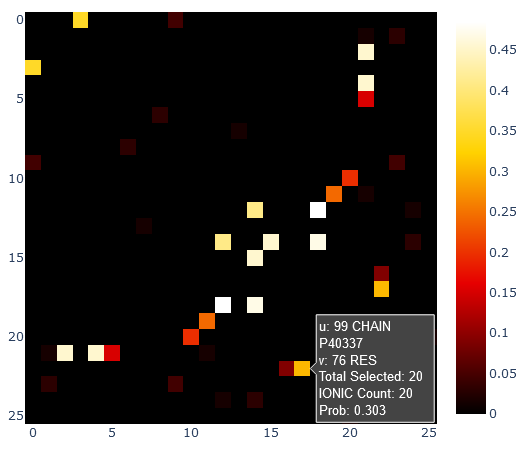
\includegraphics[width=0.5\textwidth]{fig/Contact_conserv.png}
    \caption{Example of \emph{contact conservation plot} showing the scores for \texttt{IONIC} and \texttt{PIPISTACK} interactions for all node types: \texttt{RES}, \texttt{CHAIN}, and \texttt{LIG}.}
    \label{fig:ex-contact-plot}
\end{figure}
\subsection{Co-Evolution of Contacts} % Rename this section, coevolution is not correct
With the importance of non-covalent interactions for conformal and functional properties of a protein, a reasonable analysis task is to analyze the conservation and specificity of interactions witin a family by observing the presence of interactions within spesific homolog structures. To achieve this, we provide a means means of classifying structures into a pseudo-taxonomy, grouping structures based on homology-aware RIN similarity. 
Typically, evolutionary relationships can be inferred by sequence similarity: using disparities between multiple residue sequences to infer the elapsed time since a common ancestor. Further structure is given to these relationships by organizing individuals into a tree to map their relationships. We utilize this concept to compare and group structures based not on sequence similarity, but rather the similarity of their respective RINs.

At the core of this approach is a means of quantifying the dissimilarity of RINs based on their graph definition and the node maps integral to hRINs.
Given a hRIN $G = (N, E)$, for homolog protein structure $x$ we define $E_x \subseteq E$ to be the set of edges observed in structure $x$. 
We continue to define the edge difference set, $D_{x,y} \subseteq E$ for two homolog structures $x$ and $y$ to be the set of edges present in either $x$ or $y$ exclusively. This can otherwise be thought of as the symmetric difference of the subgraph edgesets:
$$
D_{x,y} =(E_x\backslash E_y)\cup(E_y\backslash E_x)= E_{x}\oplus E_y
$$
Visulization of this operator is shown in Figure \ref{fig:graph-diff}. Observe, edges are considered to be shared between two graphs if their incident nodes have the same labels. We are able adapt this notion thanks to the node maps created with the MSA, and may avoid using more complex and computationally expensive notions of graph similarity. Additionally, the result may have node set of the result will be the union of the two graphs. 
\begin{figure}[ht] % replace with [H} if position is causing problems.
    \centering
    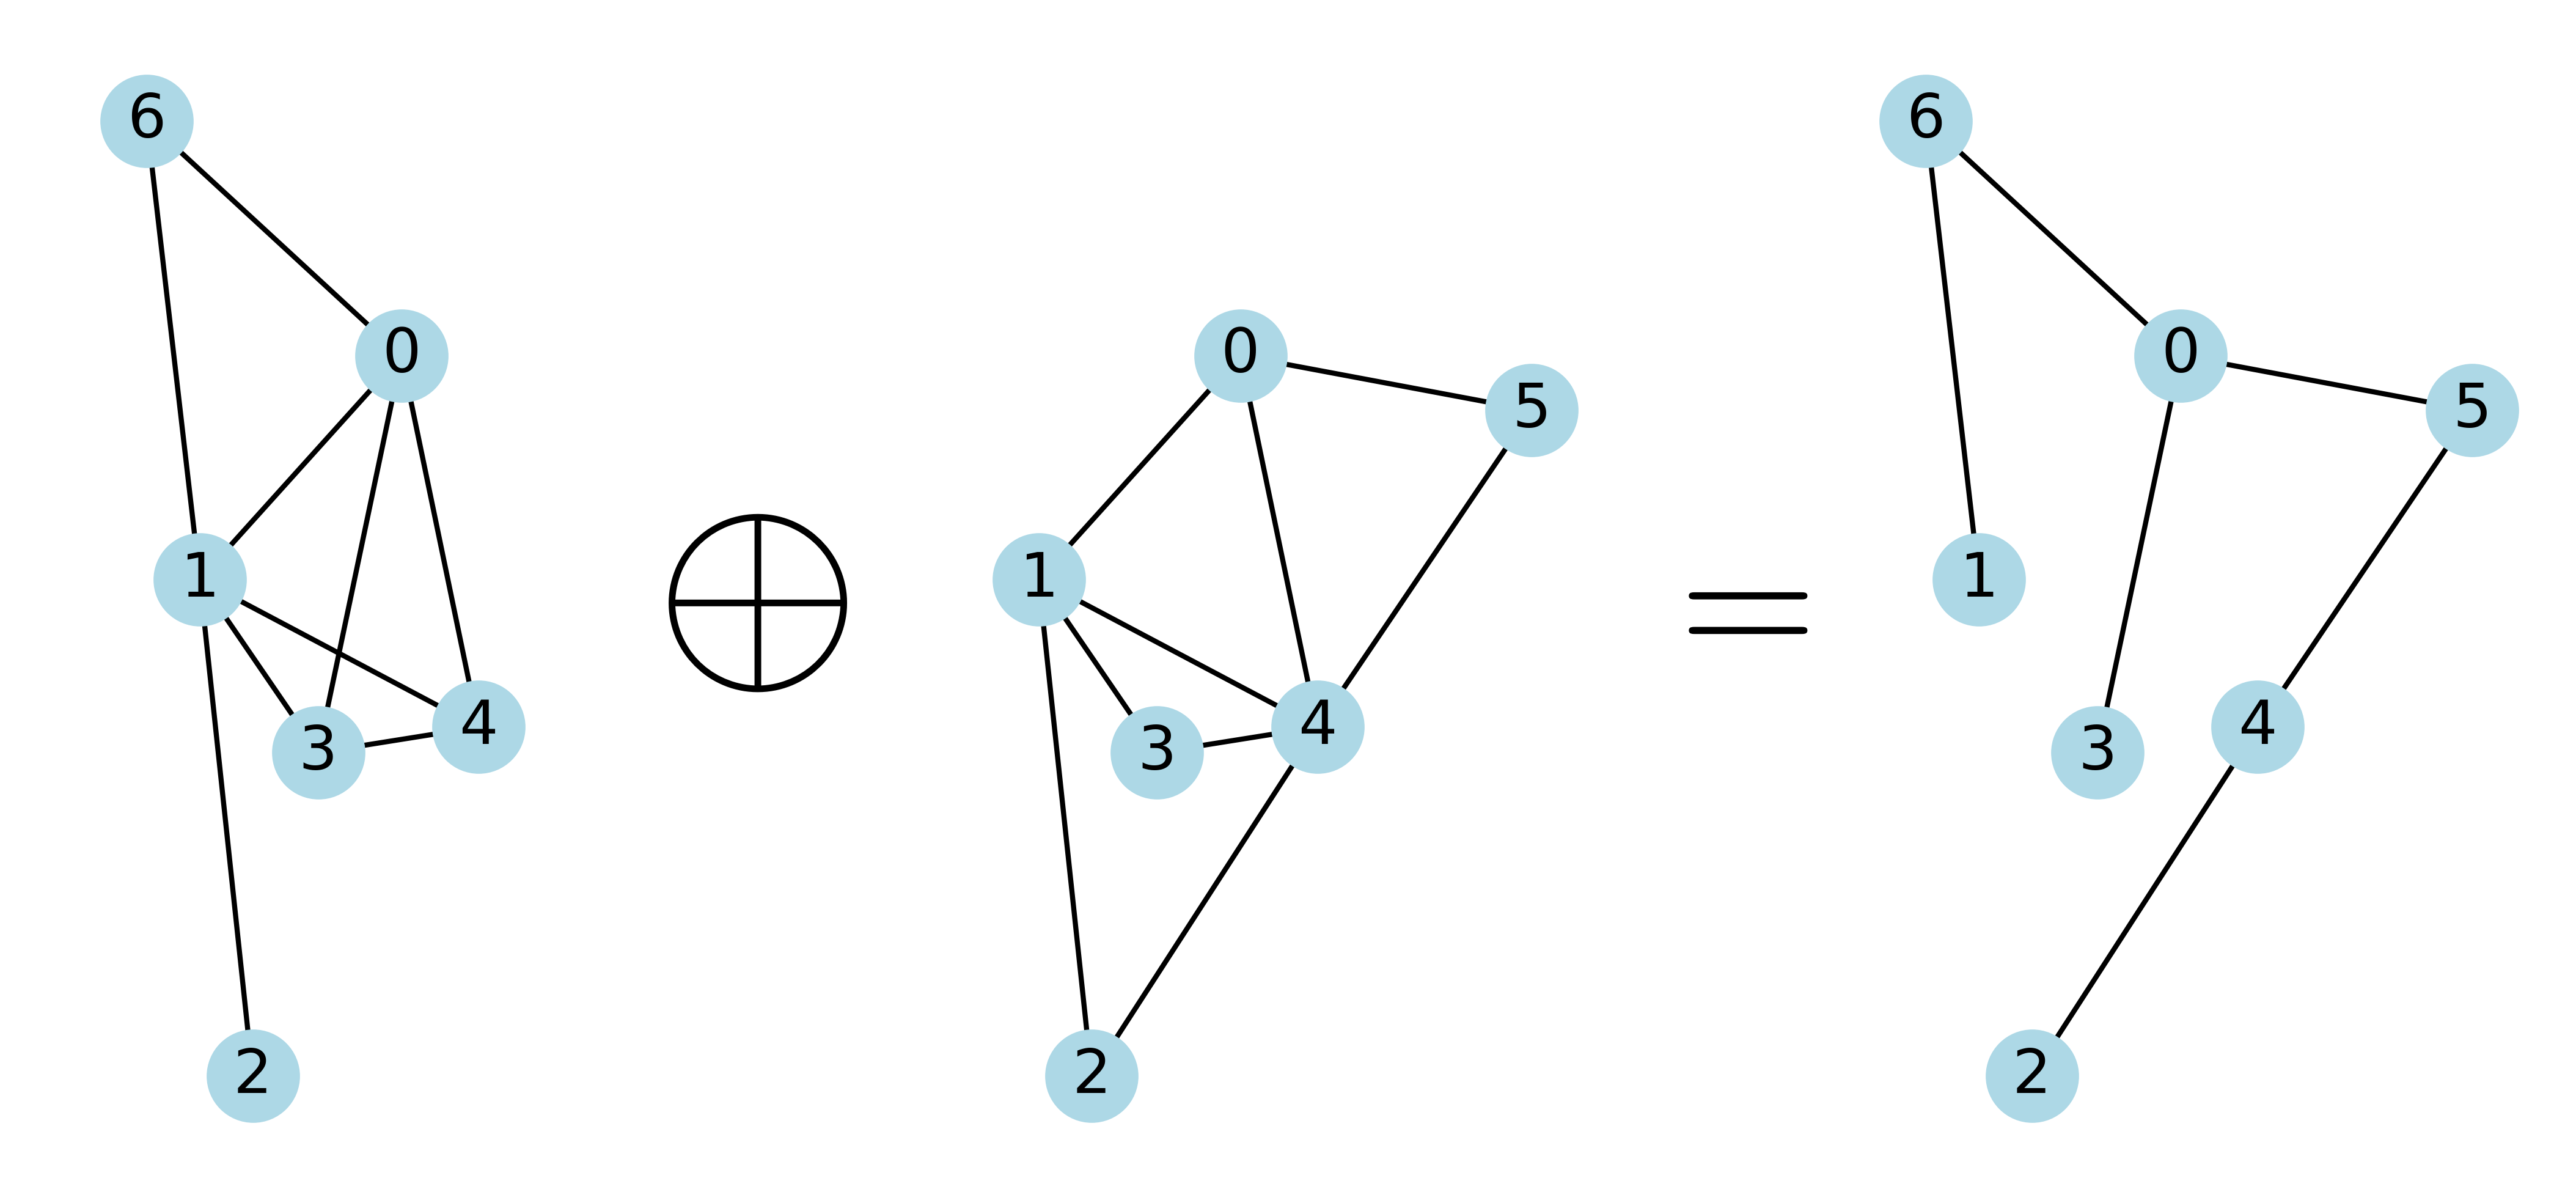
\includegraphics[width=0.5\textwidth]{fig/graph-diff.png}
    \caption{Example of the graph \emph{Symmetric Difference} (XOR) operator on graphs.}
    % For $A,B \subseteq G$, we consider edges in $A \oplus B \subseteq G$ to contribute to the distance between $A$ and $B$.
    \label{fig:graph-diff}
\end{figure}

With this we define both a unweighted and weighted pseudo-distance\footnote{This cannot be called a true distance metric, as the triangle inequality does not neccessarially hold. However, does not represent a significant issue for practical issue.} to quantify the dissimilarity of homolog chains based on the interactions the admit.
$$
d(x,y) = |D_{x,y}| \quad\text{or}\quad d(x,y) = \sum\limits_{e\in D_{x,y}} p(e)
$$
This is also referred to as Hamming distance, though it is worth noting that the weighted version in this context differes from most uses of the Weighted Hamming Distance, where the difference in edge wieghts between the two different graphs are summed. Here the edges, if they are shared between the two subgraphs, will have the same weights, and will not contribute to the distance.

The ladder weighted variant will penalize more discrepancies of highly conserved edges - considering homologs with edges , where the unweighted variant  considers only the number of unshared edges significant. 
The type of analysis being performed should inform the choice between the two. Studies of contact conservation will desire that structures that admit highly conserved edges will be grouped closer together in the resulting taxonomy, while studies of specificity will value shared novel or uncommon edges more important when grouping structures.

With the distance metric defined, the sequences organized into a rooted tree, or deprogram, using the popular unweighted pair group method with arithmetic mean (UPGMA) method. 
This is an iterative method, employed here to create a heigharchial clustering of structures based on non-covalent interactions of interest. At each iteration, the method defines a distance between groups of examples based on the average inter-group distance:
$$d(X,Y) = \frac{1}{|X||Y|} \sum\limits_{x\in X} \sum\limits_{y\in Y} d(x,y)$$

This is referred to a pseudo-taxonomy because it does not aim to capture inferred evolutionary relationships, rather group structures based on the similarity of the non-covalent interactions the admit. This is useful for finding patters of contact conservation or specificity. For example: conformal variations of a protein complex may give rise groups of variably conserved interactions. 
\todo{replace fig with example dendrogram}
\begin{figure}[ht] % replace with [H} if position is causing problems.
    \centering
    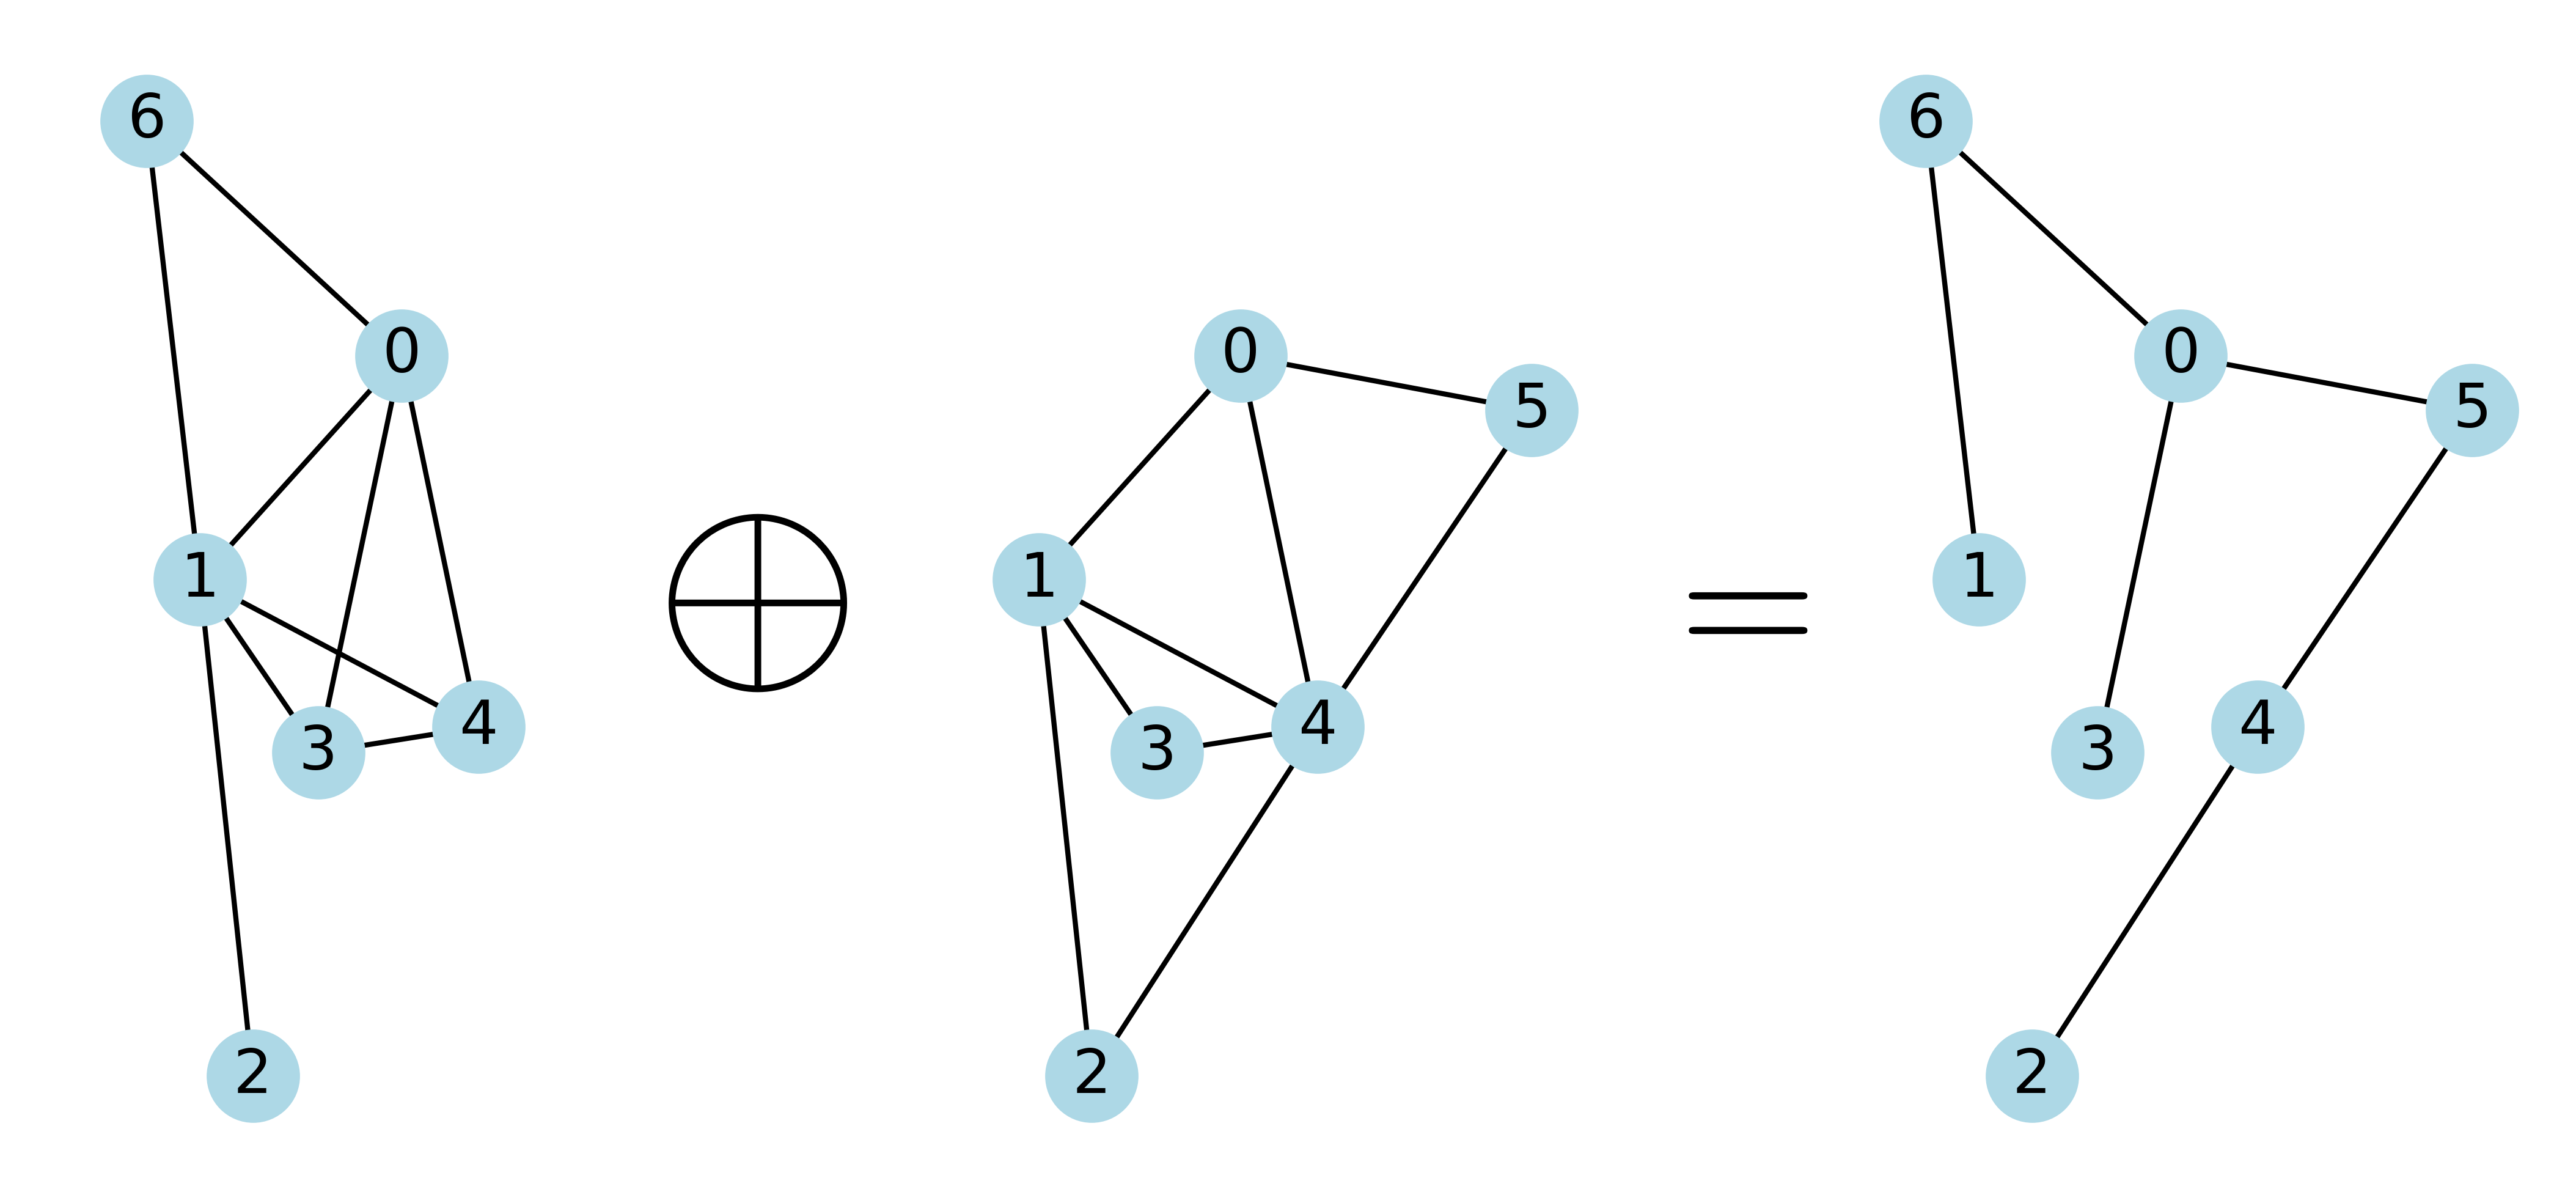
\includegraphics[width=0.5\textwidth]{fig/graph-diff.png}
    \caption{Example of dentrogram created to created structural similarity based on residue interactions.}
    \label{fig:struct-dendro}
\end{figure}
\section{Discussion And Applications}
\subsection{PAS Domain - Binding Specificity}
\subsection{Elongin C - VHL Interaction}
% Subsection Introduction
In this section, we demonstrate the utility of HomologyRing to quickly give structral insight to a particular protein family and the complexes it forms. 
Study of interactions contributiong to the formation of protien complexes is done by considering the inter-chain interactions with in a hRIN. 
The inter-chain interactions are edges that connect a node representing a family of residues, here reffered to as `residue nodes', to nodes that represent an entire entity or protein chain other than the homologs identified through the BLAST search, identified here as `chain nodes'.
We will use the interactions formed by the RNA Transcription Factor B complex, to demonstrate these capabilities. 

Transcription Factor B, also known as SIII or simply Elongin, is a protein complex responsible for promoting RNA polymerase II elogation by suppressing the function of arresting sites within a transcription window \cite{Chen2023}. In this sense it has been identified as an elongation factor regulating transcription by RNA polymerase II. Transcription processes are most commonly thought of as being regulated by initiation factors. However, regulation of the process during elongations is increasingly understood as being significantly important. The Elongin complex is seen to be dynamic and known to have several other interacting factors affecting elongation behaivor. % https://www.nature.com/articles/s41594-023-01138-w#ref-CR8 % CUL5–RBX2 complex
We will primarially focus our discussion on ELOC: using it as a query inorder to build an hRIN with HomologyRing to observe inter-chain interactions in the Transcription Factor B (SIII) and related complexs. 
Comparing structural insites gained through HomologyRing to results from the literature will be used to demonstate the usefulness of the tool and information contained in the resulting hRINs.  

%% Move this to where we start talking about the pipeline being run
It this case, it is worth noting that we are not primarially concerned with the construction of a family of homolog proteins per se. Rather, we can expect a BLAST search of the PDB to return many ELOC orthologs, or human isoforms (of which there are three \cite{Chen2023}), resulting in a family of high sequence similarity, but may very considerably in the entities present in each complex structure. % stub
%%% END STUFF TO MOVE

%% Complex introduction
Before detailing the running of the pipeline and intrepeting the resulting hRIN, we pervide some context for the significance of Elongins structure and function. 
The SIII compex is composed of three elongins: A, B, and C and are highly conserved in Eukaryotes. 
These elongin protein products are respectively refered to by their short gene names: ELOA, ELOB, and ELOC.
Behaivor of the SIII elongation factor is well studied experimentally, and has enjoyed a lot of attention. However, much of its function on a mechanistic level is yet to be fully understood. 
% ELOA structure and function
ELOA as a monomer has been seen to promote elongation by RNA Pol II alone \cite{Aso1995}, as ELOA is the is responible for binding in the SIII Elongin complex with the larger RNA Poly II complex where Elongins B and C are regulatory subunits. Additionally, ELOB and ELOC are seen to form a subcomplex independent of ELOA. \cite{Chen2023}, and as will be seen later, is under represented in structures of complexes in the PDB containing ELOC. 
As a result, we will primarially discuss the interaction between ELOC and ELOB. 
% ELOB structure and function
ELOB (seen in \ref{fig:SIII-structure}), 
Ubiquitin-like protein %https://www.nature.com/articles/s41594-023-01138-w#ref-CR14
% Globular core
% Disordered tail at X-terminus
% ELOC structure and function
SCF ubiquitin ligase subunit Skp1 % ??? I think this is describing a different complex
% https://www.nature.com/articles/s41594-023-01138-w#ref-CR8
Seen to promote the activity of ELOA %https://www.nature.com/articles/s41594-023-01138-w#ref-CR14

Figure \ref{fig:SIII-structure} shows an ELOB - ELOC complex interacting with a portion of pVHL.

We show a complex of ELOB, ELOC, pVHL incomplex with a region of HIF in Figure \ref{fig:SIII-structure}.
\begin{figure}[ht] % replace with [H} if position is causing problems.
    \centering
    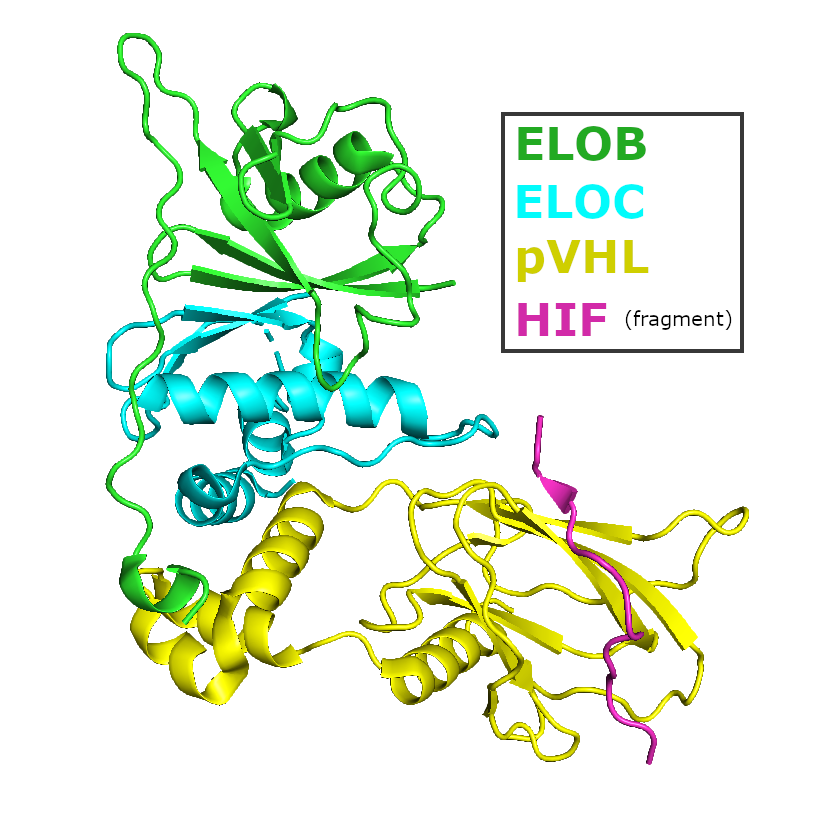
\includegraphics[width=0.5\textwidth]{fig/SIII_1LM8.png}
    \caption{PDB: 1LM8; Complex of Elongin B,C with pVHL and HIF-region \cite{Min2002}.}
    \label{fig:SIII-structure}
\end{figure}

% Introduce pVHL

Notabale regulation activity comes from the SIII interaction with the Von Hippoel-Lindau Tumor Suppressor Protein (pVHL) which is coded for by the VHL gene. Elongins B and C have are known to interact with pVHL in the SIII complex. pVHL, in this interaction is seen to inhibit transcription elongation. 
%pVHL context
The pVHL product is well-known a regulator of many different pathways and known to interact with several other proteins \cite{Tabaro2016}. However, the protein has recieved much attention for its role as a tumor suppressor \cite{}, and owes its name for its associated Von Hippel Lindau syndrome -- an inheritable genetic mutation to the VHL gene which is associated with a very high propensity for tumor devlopment in many highly vascularized tissues throughout the body. 

At the protein level, VHL is known for its role in regulating tissue response to hypoxic, or low oxygen, conditons. 
Spesifically, pVHL is seen to be contribute the the ubiquitination of hypoxia-inducible factors (HIFs). 
HIFs are transcription factors, or proteins that bind to spesific regions of DNA to regulate their transcription.
They are a key component the process through wich mamilian cells respond to hypoxic conditons, or prolonged leveles of low oxygen. 
Hypoxia is highly relevant to many forms of cancer, as tumos growing and eventually cutting themselvs off from blood supply in their interior are a common pattern. HIF, working as a transcription factors, can promote the thranscription of various different genes which may serve to mitigate the effects of hypoxia, correct it, or signal for the destruction of the cell. One known mechanism for addressing the issue of hypoxia in tissue is signialing for the additional vasculature, thus increasing the supply of blood and oxygen to the area. This behaivor is highly characteristic of the tumors seen in VHL syndrome, occuring in highly vascularized areas such as parts of the brain, retina, and spine, among others. % https://en.wikipedia.org/wiki/Von_Hippel%E2%80%93Lindau_tumor_suppressor#cite_note-Ben-SkowronekKozaczuk2015-5

%pVHL structure

% funtion , types of mutations to VHL
Healty pVHL, in complex with ELOB and ELOC,  tags HIFs with Ubiquitin, signiling for their destrction, and thus working to down regulate a tissues hypoxia response. Mutations to the protein such as the ones seen in VHL syndrome



%%% pVHL HIF interaction, structure
HIF contains a highly conserved proline containg region which is the binding substrate where the HIF will bind to pVHL. 
In hypoxic enviroments, the prolines in this region will experice hydroxulation, a post translational modification where proline will gain an hydroxyl groub on the sidechains gamma carbon. This modification enables pVHL-HIF interactions and subsequent ubiquinition of HIF, a process that eventually leads to the destruction of the HIF, freeing the gene region to which it was previously bound. This process is critical for allowing cells to variably express genes based on the amound of oxygen avaible to the cell, allowing for behaivoral changes that allow for its survival like angiogenisis or alternatively programmed cell death in low oxygen senerios \cite{Carmeliet1998}. 

%pVHL function (breakdown)
% pVHL interaction sites

This well-studied complex has recieved much attention for its role in several cancers. 
% This should be moved somewhere else --- possibly in the section where the PDB database is introduced
% Write a shorter blurb explaining this idea to go here
It is important to note that a homology search of the PDB does not neccessarily return a set of distinct, evolutionarily related sequences. Instead, the Homology search as implemented by BLAST reutrns sequences with high sequnce similarity to the query. This will most likely many different structures for the same protein, as the PDB may contain many structures for the same protein.
This is desiarable behaivor, given that tese different enteries may correspond to the protein in different biological contexts, with differences in temprature or pH; additionally a protein of interests may form different complexes with many interactors, or experience conditional conformal variations. 
All of these factors influcence the structure and corresponding RIN of a protein. Given this networks with noteworthey differences in topology can be seen to represent the same protein chain. By coreating a hRIN for a sigle protein, we obtain a single object that may be used to represent a protein that captures both  variations and conserved features of a protein.


%PIPELINE AND RESULTS
The preceding sub-sections serve to illustrate the many complicated interactions in which ELOC participates. Each of these interactions is quite nuanced, and a complete picture of all possible interactions and their functioning at a molecular level is a very time consuming process to come to understand. Furthermore, in this case there is still much that remains not compleatly understood. Here we will utilize HomologyRing to quickly an object capturing structural information about protein-protein interactions at the residue level. This may be used as an overview, providing researchers a quick introduction to wich sites and compounds are involved in interactions in a protein family, or as a technical, well defined mathematical object, wich could be used for more quantitive analysis. In this section we will demonstrate the former, using HomologyRing to quickly gain initial insight in to the Elongin Complex.

The  section as a detailed account of the considerations commonly made when analysing hRINs; aswell as challenges presented by the data, and how tools provided by HomologyRing can adress them. Namely, the propensity and biological significance of different types of interactions, means that a filtering process can greatly aid visualization. Furthermore, variation in the protein chains present in each structure included in the family needs to be considered when conserned with the conservation of interactions.

After initiating the pipeline to build the hRIN, we will first address the different protein chains included in the set of structures. 
Since we are here concerned with interactions of multiple protein chains, we are required to restrict the use of the pipeline in this case to a homology search of the PDB, as predictions avaible in the AlphaFold Database are limited to single chain structures, preventing the study of inter-chain interactions. 
Bias in the PDB in some ways limit the usefullness of the quantitive information in the graph. The probability weights in the inter-chain edges of the graph are heavily influenced by the frequency with which published experimental structures have captured any given two entities in a single structure. As discussed, the size of the greater complex associated with Elongin is dynamic and highly variable. 
Presense of particular entities in experimental structures is also influenced by factors such as interest in particular aspects of a complex within the research community and difficulty of chrystialization. 
%Both of these factors distance the edge weight data from being effective measures of the propensity for an entities interaction in a biological context and such biases should be considered for more statistically rigorous analysis aimed at studying such interactions.

We begin our analysis of the Elongin complex by centering our focus on the ELOC chain, using it as our query structure. And with this we may begin spesifying parameters to construct a HomologyRing quert. Spesifically, the query chain is taken from the \texttt{AUTH C} chain of the PDB structure \texttt{1LM8}, which is a x-ray chrystal structure of the ELOB-ELOC dimer in complex with a fragment of pVHL \cite{Min2002}. The corresponding query sequence is 88 residues long, and maps to uniprot accention {Q15369-2} isoform, differing from the cannonical sequence by an omission of 16 residues from the N-terminal, or beginning of the sequence. 
The PDB Europe Knowledge Base lists 164 structures in the PDB mapped to the ELOC Uniprot gene: \texttt{Q15369}. However, many more close homologs exist with high sequence similarity.
Creating an hRIN win an aim to create a comprehensive account of all ELOC structures in the PDB is perfectly feasible with the RingHomology pipeline and can capture infromation from all 164 structures comprising more than 500 MB of information in a few minutes on consumer hardware. However, for the sake of simplicity of visuilization we limit the homolgy search to just 128 results here. Since in this use case we aim to perform a narrow analysis on spesifically the ELOC gene, we set a conservitive E-value theshold for the homology search of $5 \times 10^{-3}$, restricting results to sequences with high pairwise similarity to the query sequence.

Running the pipeline quickly constructs an hRIN. In this section we will use the analysis tools included in the HomologyRing package to explore the information contained in this object on a sequence, structural, and network level. Firstly, examining the amino acid sequences belonging to each homolog chain is an excellent way to begin intrepreting information about the family. The MSA created by the pipeline is used internally for the definition of nodes in the network, and its visualization serves as a useful aid for understanding the hRIN. Figure \ref{fig:eloc-msa} shows a representation of the MSA where residues in each homolog sequence is colored according to CLUSTAL colors, which groups amino acid residues according their chemical and physical properties, This is covered in more detail in \ref{sec:contact-mask} with the exception that here no contact information is displayed. \todo{Finish section detailing the MSA analysis contact plots}
As seen in the figure, this family has a high degree of sequence identiy. This is an anticipated result due to the number of ELOC enteries in the PDB and restrictive E-value set when running the pipeline. The exact identity of the protein chains are discussed shortly in this section. The MSA shows high identity in the majority of columns, with a handful of 1-2 residue deletions introducing gaps, and only a few notable substatutions. 
Residues 35 - 42 are clearly seen to have low occupancy compared to the rest of the residues. Referencing structures in the family as well as Interpro entries, show that the region correspond ot a hairpin turn of variable length. These are common regions of variation, and as we will see, correspond to a region with little significance to inter-chain interactions seen in the PDB complexes. \todo{Change if this is wrong}
The high identity in the family is useful reducing the overall complexity of the resulting hRIN, which aids in simplifying the subsequent analyses.

%% MSA Figure
\begin{figure}[h!] % replace with [H} if position is causing problems.
    \centering
    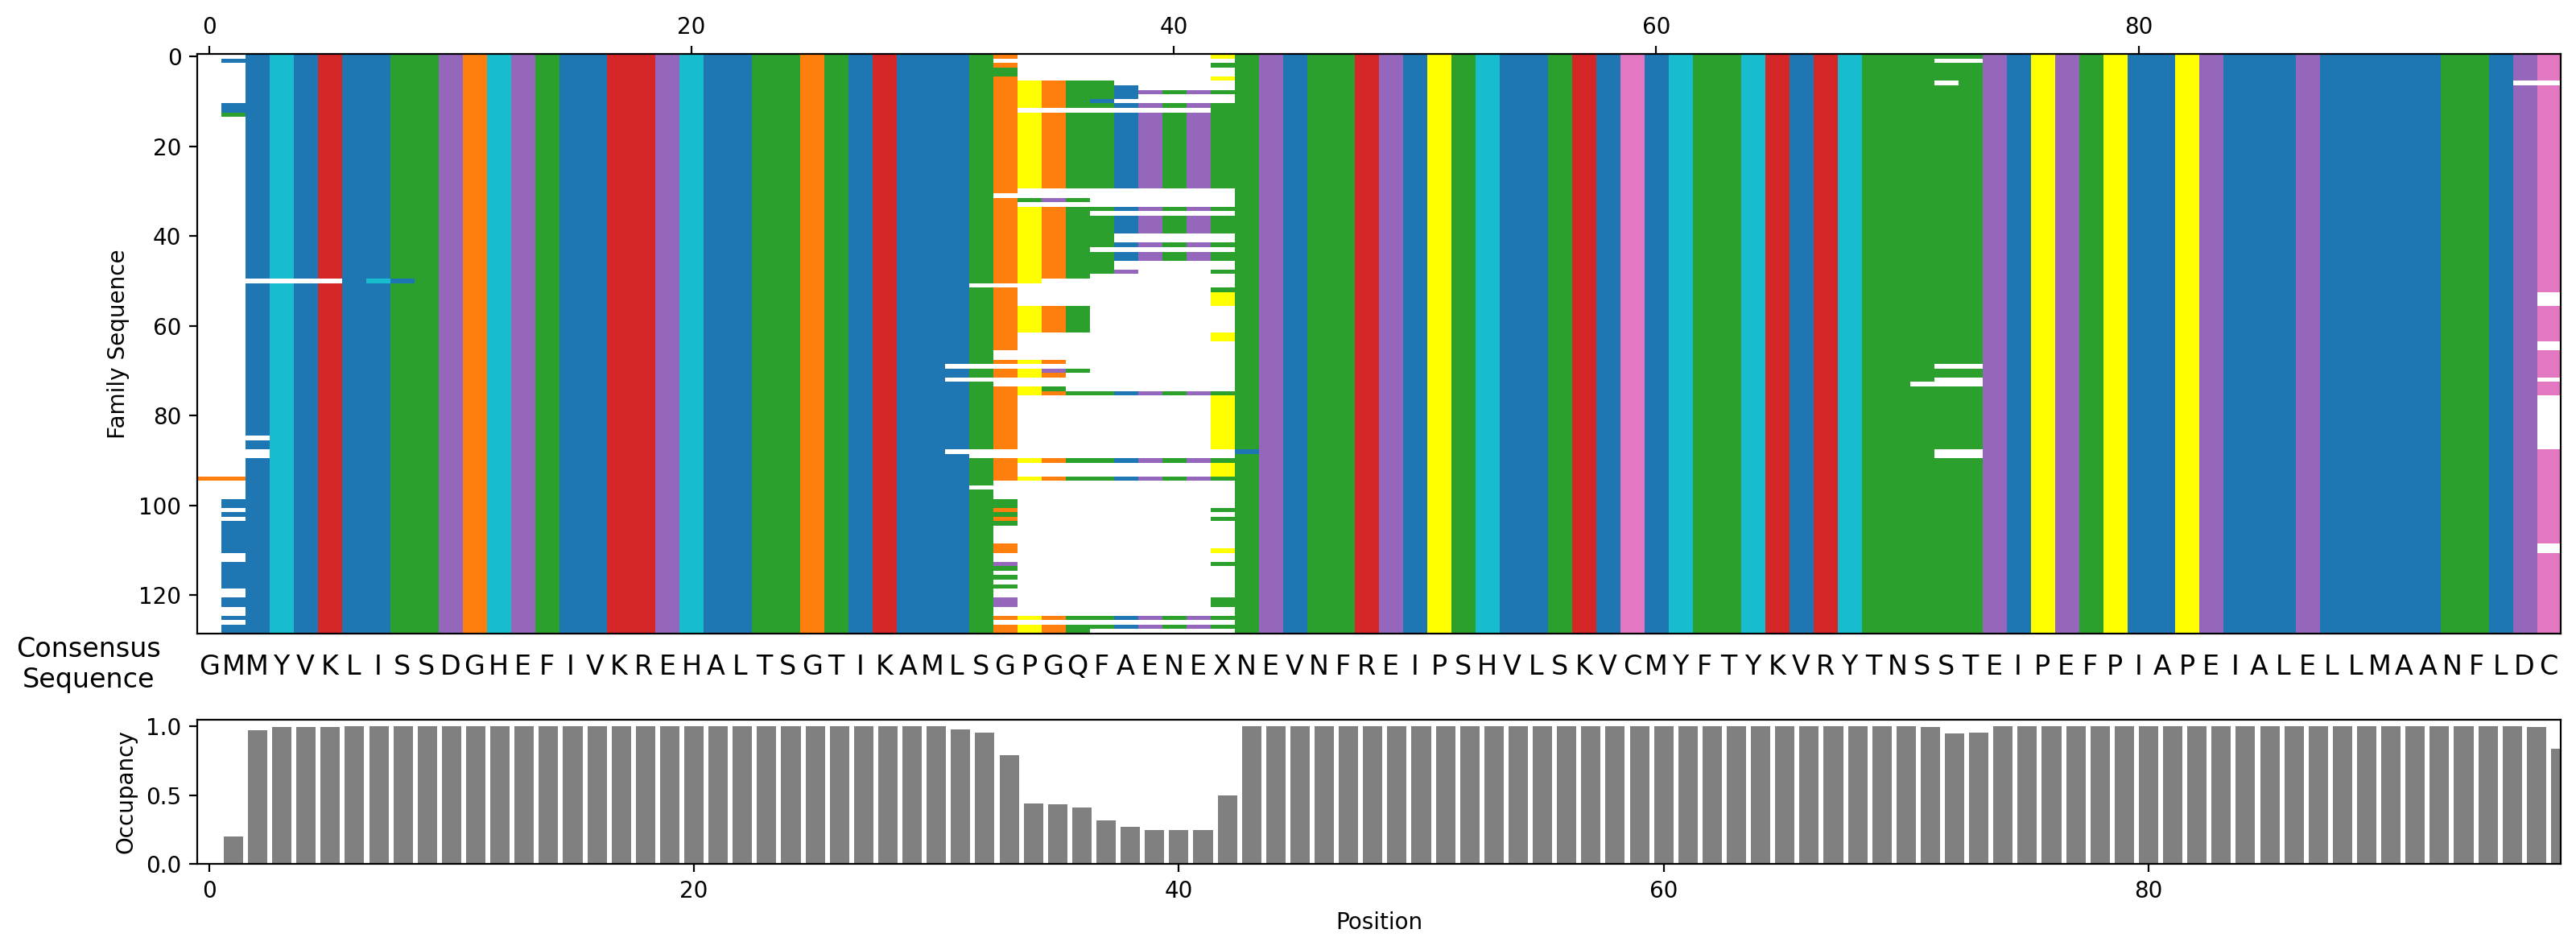
\includegraphics[width=\textwidth]{fig/ELOC-MSA.png}
    \caption{Representation of a multiple sequence alignment for the ELOC family. Created as part of the HomologyRing pipeline with Clustal$\Omega$}
    \label{fig:eloc-msa}
\end{figure}

%% Table of common protein chains
As stated, a primary aim of this analysis is structural insight into inter-chain interactions. To begin, we will summarize which protein chains are present in the families structures. This gives indication of wich proteins are commonly observed in complex with homologs of our query in the PDB and wich interactions are captured by the network. Table \ref{tab:eloc-chain-count} provides an overview of the presence of protein chains in the structure collected to form the family. HomologyRing exposes this information orginally collected from CIF metadata and includes additional information on ligand presence and are provide reference for detailed information associated with nodes in the network. 

ELOC\_HUMAN, despite being used as the query seqeunce, is only listed as present in $98.2\%$ of structures. This is due to close homologs like ELOC\_MOUSE comprising a small handful of the homolog chains included in the family.  
We also observe that the distribution of protein chain counts has a long tail. Truncated from Table \ref{tab:eloc-chain-count} was 30 different proteins that appeared in no more than 2 structures. Some are the close homologs, as previously mentioned, while others are lesser studied proteins associated with Elongin or RNA Poly II. 

\begin{table}[h!] % Use [H] for exact placement, if necessary
    \centering
    \begin{tabular}{l c c c}
    \textbf{Gene} & \textbf{Chains} & \textbf{Structures with Chain} &  \textbf{Structures with Chain (\%)} \\ \cline{1-4}
ELOB\_HUMAN & 158 & 63 & 98.4\% \\
ELOC\_HUMAN & 124 & 59 & 92.2\% \\
VHL\_HUMAN & 78 & 39 & 60.9\% \\
CUL2\_HUMAN & 38 & 18 & 28.1\% \\
RBX1\_HUMAN & 24 & 14 & 21.9\% \\
FEM1B\_HUMAN & 19 & 10 & 15.6\% \\
APBP2\_HUMAN & 16 & 5 & 7.8\% \\
PEBB\_HUMAN & 15 & 3 & 4.7\% \\
BRD4\_HUMAN & 15 & 8 & 12.5\% \\
CUL5\_HUMAN & 14 & 2 & 3.1\% \\
RASK\_HUMAN & 6 & 3 & 4.7\% \\
HIF1A\_HUMAN & 6 & 3 & 4.7\% \\
\textbf{OTHER} & 77 & 34 & 53.1\% \\
    \end{tabular}
    \caption{Number of occurences of each the most common protein chains in the family constructured by the HomolgyRing pipeline. Family consists of 129 homolog chains from 64 different unique structures from the PDB. Structures may contain more than one protein chain transcribed from the same gene. Number of structures in the family that posses the protein corresponding to the given gene are also indicated. This table serves to give an overview of wich interchain interactions are well captured within the constructed hRIN.}
    \label{tab:eloc-chain-count}
\end{table}

The high rate of ELOB inclusion indicates that the hRIN serves well to capture the minimal Elongin ELOB - ELOC complex and pVHL and CUL2 are present in an appreciable proportion of structures -- $60.9\%$ and $28.1\%$ Respectively. Given this, we will explore information contained in the hRIN about the ELOC - ELOB, ELOC - pVHL, and ELOC - CUL2 interactions. When studing the significance of inter-chain interactions within a family, a percise notion of `conservation' is needed. A naieve approach would be to weight interactions according to the number of times it is observed within a family. However, key interactions with a chain that is in only a minority of structures will be labeled as poorly conserved with such an approach. To address this, we use a normalization approach that considers if an interaction is possible based on the chains present in a file, which is detailed in Section \ref{subsec:def-conservation}. The effect of this normalization is clearly seen in figure \ref{}. 

%% Possibly speak about intra-chain contacts
%% See if there are regions of variable contacts in mobile regions
Moving on the second major consideration guiding this analysis, the spesific interactions, we begin by observing the interactions between the most prelevant proteins, ELOC and ELOB. Either prior knowledge of the family or exploratory analysis of which interaction types are relevent and limiting visualizations accordingly is often helpful. The different types of interactions residues may participate in are generally seen to be differently distributed in the case of intra-chain, inter-chain, and chain-ligand interactions; and Table \ref{tab:eloc-inter-counts} shows this to be the case for this family. Notable types of interactions may only occur between specific, and often reletively rare, amino acids. Consequently, the presence of such an interaction often confers a significant structural function, and the conservation of the interaction will usually correlate with the high conservation of the participating residues in homologous sequences. %% This really does not need to be mentioned here.
On the other hand, interactions like Van Der Waals Forces, or hydrogen bonding are more proliferic, capable of occuring in most if not all amino acids. Such interactions are increadibly important for the conformation of individual protein chains as well as the formation of complexes, however, if they are not of paritcular interest, their abundance can complicate analysis. 
With this in mind, we 


\begin{table}[h!]
    \centering
    \begin{tabular}{l c c c}
        %\hline
        \textbf{Row Label} & \textbf{Intra-Chain} & \textbf{Inter-Chain} & \textbf{Chain-Ligand} \\ \hline
        HBOND & 7347 & 1550 & 15 \\ 
        VDW & 7431 & 3789 & 36 \\ 
        PIPISTACK & 595 & 472 & 0 \\ 
        IONIC & 174 & 214 & 0 \\ 
        PICATION & 54 & 36 & 0 \\ 
        PIHBOND & 8 & 7 & 0 \\ 
        METAL\_ION & 0 & 0 & 2 \\ 
    \end{tabular}
    \caption{Example table with 3 labeled columns and 7 labeled rows}
    \label{tab:eloc-inter-counts}
\end{table}

We may further filter the data provided by HomologyRing used to create Table \ref{tab:eloc-inter-counts} to consider only spesifically the inter-chain contacts between ELOC and ELOB chains. Between the two chains of interest there are the following interactions: 1117 VDW, 605 HBOND, 235 PIPISTACK, 44 IONIC, and 25 PICATION interactions.

There are three primary regions of ELOC that constitute its interface with ELOB: a continuous $\beta$-sheet, small region of contact in a central hairpin, and a disordered C-terminal region (see Figure \ref{fig:SIII-structure}). 
To demonstrate the ability of HomologyRing's analysis tools, we examine one of these regions in particular as an example. 
%% Highly conserved PIPISTACK interactions in positions 11 and 13
%% Hydrogen bonding stabalizing the primary interface between ELOC and ELOB
The primary interface between ELOC and ELOB occurs between two parallel $\beta$-sheets, nodes 11 - 17  in the hRIN which correspond to residues 26 - 32 in ELOC\_HUMAN,  UniProt: Q15369. The family consensus sequence is GHEFIVK which has 100\% identity with the Uniprot canonical sequence. 
HomologyRing allows us to visualize subgraphs of the constructed hRIN, allowing for the close examination of which interactions, or edges in the hRIN are most significant in this region.

%% Figure
%% MSA Figure
\begin{figure}[h!] % replace with [H} if position is causing problems.
    \centering
    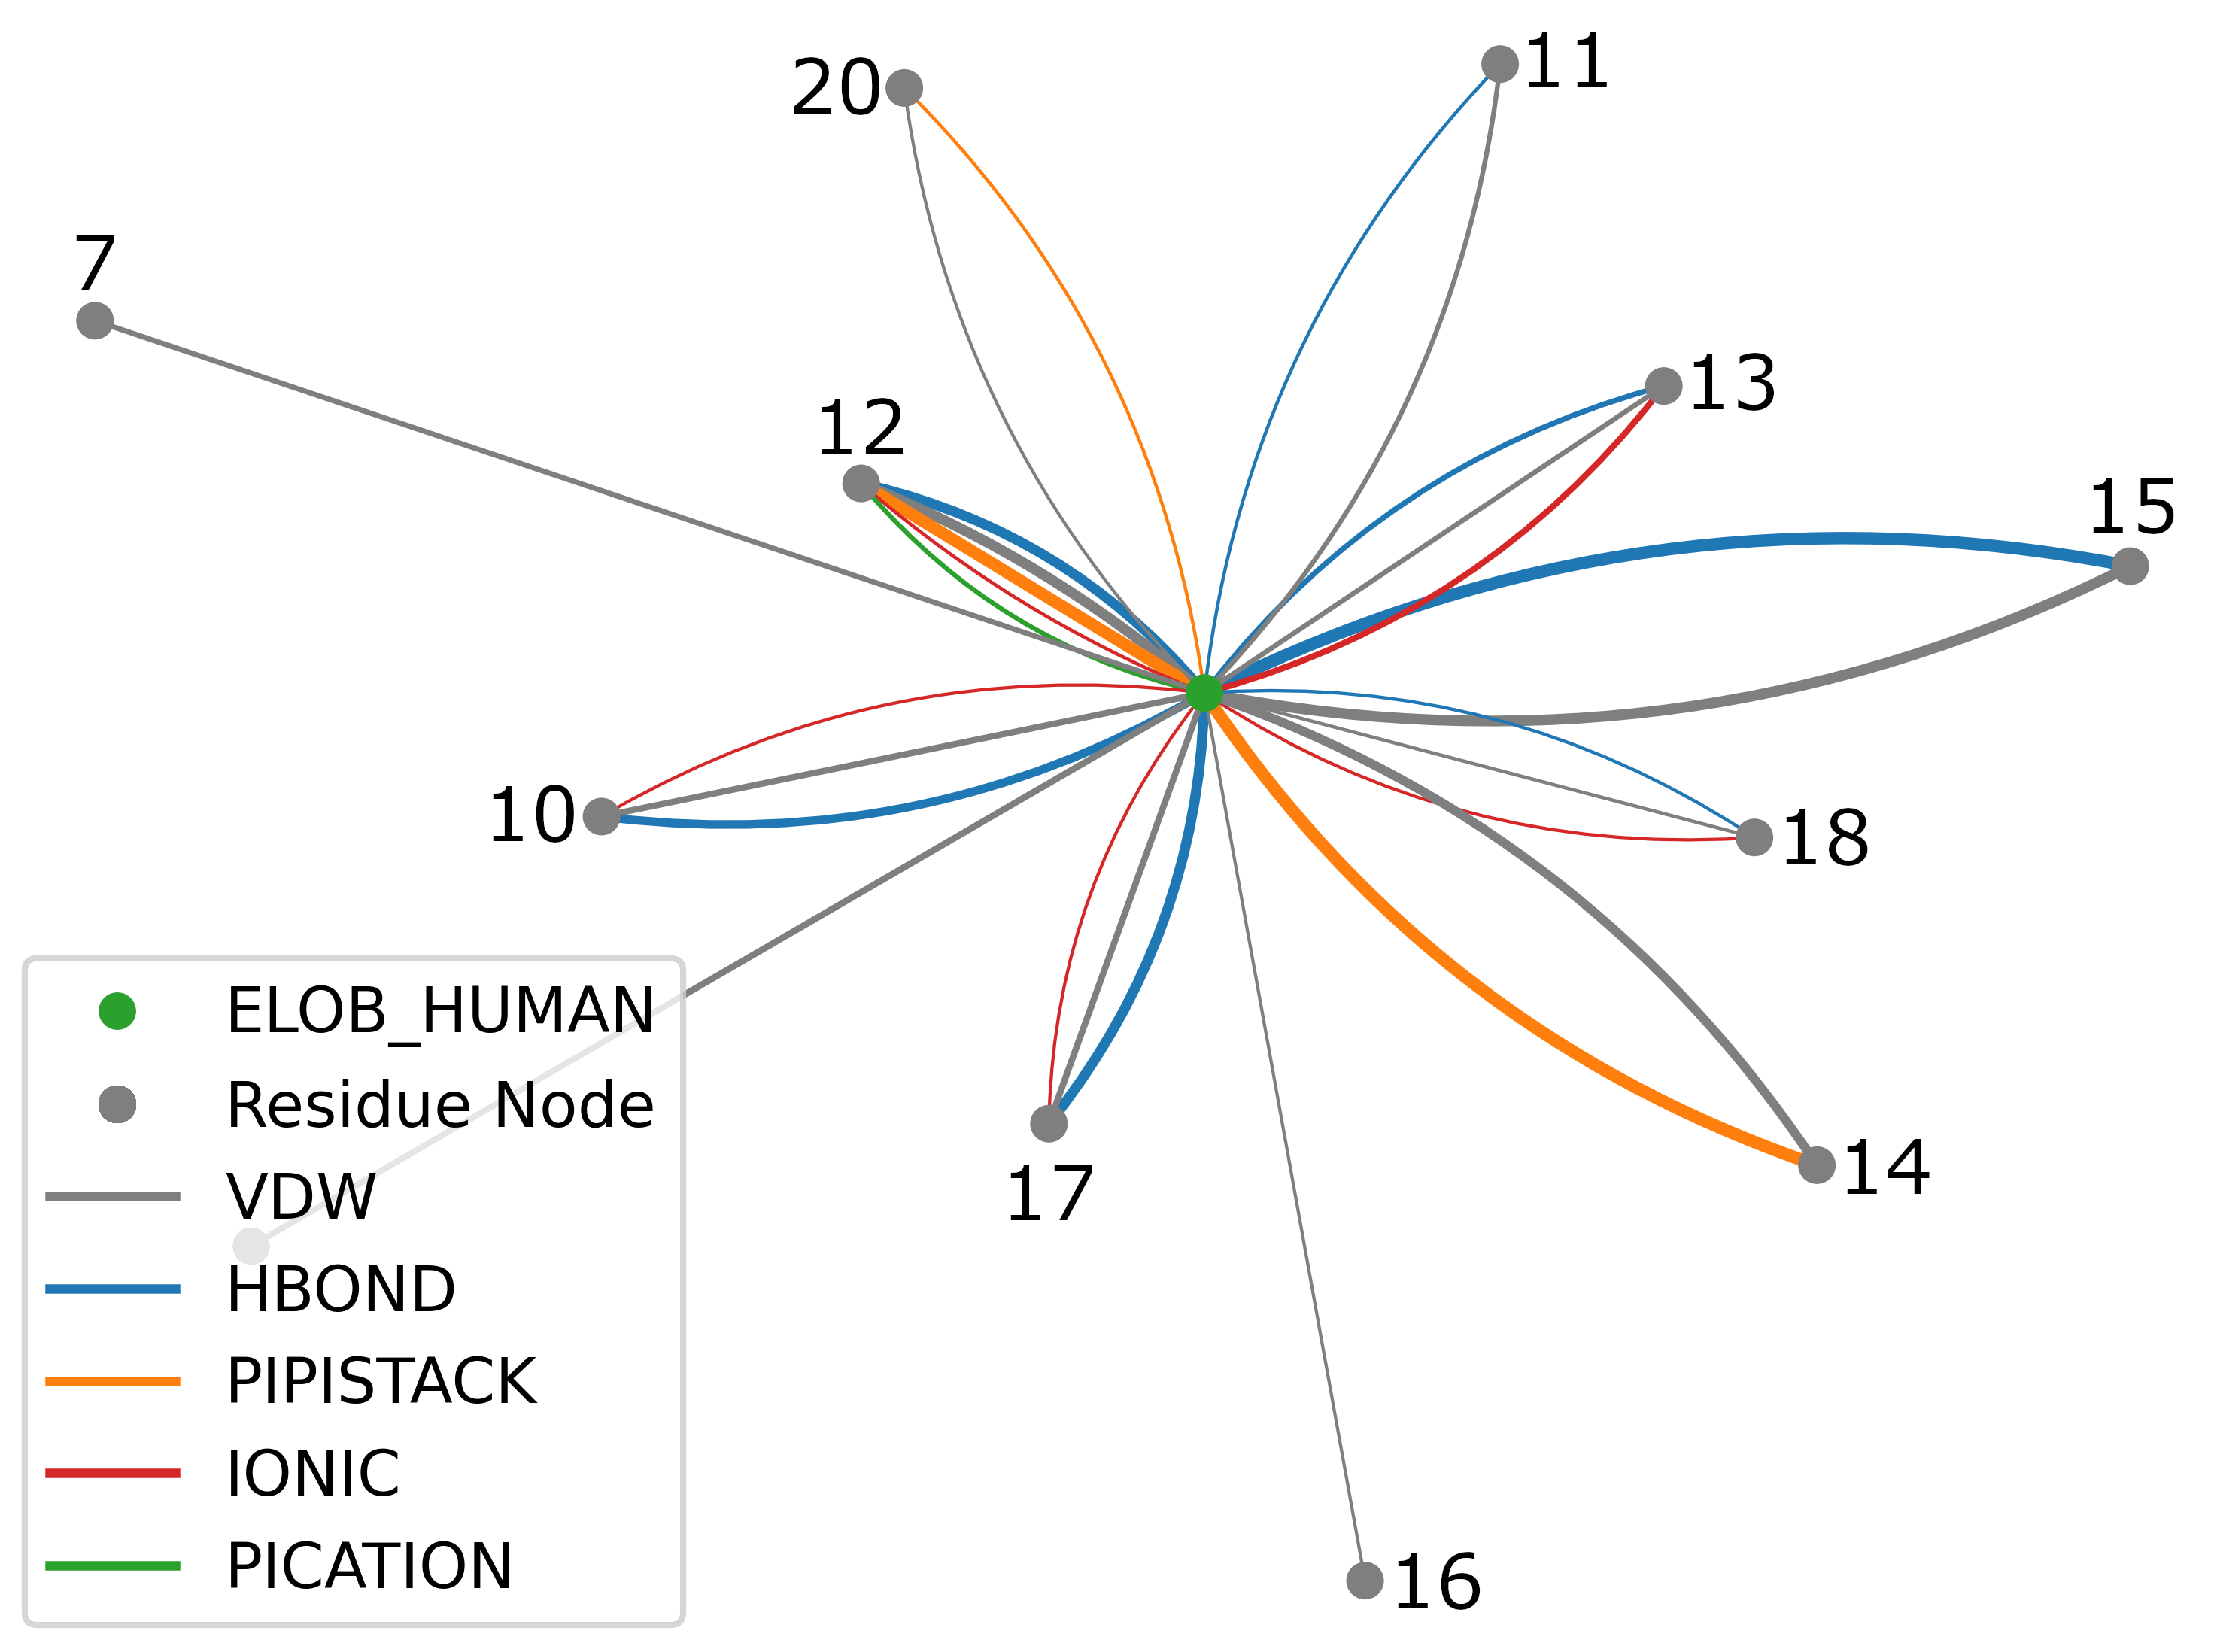
\includegraphics[width=\textwidth]{fig/eloc-bsheet-net.png}
    \caption{Sub-network of hRIN created for studying the inter-chain interaction between ELOC\_HUMAN and ELOB\_HUMAN. Further filtering was performed to consider only residue nodes 11 - 17 corresponding to a $\beta$-sheet comprising the primary stabilizing component of the ELOC - ELOB complex. Where a full network is too large to effectively visualize, this network clearly displays the the degree to which different inter-chain interactions are conserved in the hRIN.}
    \label{fig:eloc-bsheet-net}
\end{figure}

The figure displays noatbly several edges with notably high probability weights, indicating highly conserved interactions in the family. Such interactions can to be intrepreded as highly significant, or key interactions in the protein family. A common inference from such highly conserved interactions with high spesificity are of significant importance to their function. In this case, binding to form a complex with a nother protein chain, which as discussed earlier, is critical for the proteins function.

The network in \ref{fig:eloc-bsheet-net} conveys at a glance information from over 64 structures and 128 distinct ELOC chians. Immediately, we can se that Many residues in ELOC forming hydron bonds and Van Der Waals interactions with ELOB is a significant 

%% Disordered terminus of ELOB held inplace against ELOC mainly by weaker VDW and HYDROGEN BOND forces

%% Getting information about the disorderd tail would best be done with ELOB as the query sequence
% Table for entities present in each homolog structure.


% 2 isoforms
% VHL negatively regulate hypoxia induced products
% What is EL ubiquitin ligase in connection to this context?
%% Substrate recognition
% VHL disease
%Hareditary form of cancer caused by germline mutations
% Highly vascular
% What is angiogenisis - not *not really needed*
% note the interaction of pVHL and HIF-A conservation between species (Maxwell(?)) -- read this on wikipedia

% pVHL ELOC interaction

The binding of pVHL to 
negatively regulates the 
A conserved region on elongin C consisting of residues 17-50 is needed for the binding of Elongin C to pVHL \cite{Ohh1999}.
%Isoforms
%A2 only expressed in the testis

Elongins are a member of the ... superfamily
Elongin A is primarily responsible for nucleotide interaction and transcription function where the other sub units serve regulatory functions.
% Talk about the interactions and the nature of the VHL as a disordered protein
% Describe VHL role in cancer
VHL owes its name with its association with a long known form of cancer inherited cancer - von Hippel-Lindau disease which has come to be associated with with the VHL gene. 
VHL functions as a tumor suppressor and has many known interactions, and though  VHL is not known to have close homologs, it interacts with other genes important for RNA transcription processes [VHLdb][sci-direct]. 
Among it's known interactions is with Elongin C, which participates in in humans is part of the Transcription factor B/SIII complex.
% Possible analysis:
% 1. Run pipeline on ELOC_HUMAN
% Run the pipeline with VHL as the query chain to see if there is conservation / variation of interaction information
We investigate the specificity of interactions between Elongin C and VHL by initiating the HomologyRing pipeline using the Elongin C present in PDB: 


\subsection{DDX}
%%% NEW INTRODUCTION
DEAD-box RNA helicases, or here otherwise referred to as members of the DDX family of proteins, are critical for many processes involving RNA metabolism and are the subject of much research due to their role in the formation of many cancers. They are responsible for ATP-dependent RNA binding and remodeling, with members assuming general and more specialized roles in RNA metabolism including: RNA duplex unwinding, 
We examine hRIN created from a set of human DDX paralogues, to examine key interactions between residues in the family, and compare the results to current literature to illustrate the effectiveness of HomologyRing to identify residues and interactions critically important for the function of a family of proteins. In this case, illustrating its usefulness in studying a verity of studies, including virology, genome protection, and cancer. (big sell)

There are DDX homologs are found in all kingdoms of life including viruses; many organisms having many paralogs. Humans are currently known to have 38 (cite)
DDX proteins are members of the helicase superfamily 2 (SF2). 
Intrensically disordered N- and C- terminal domains exhibit high sequence variability within the family, which may contain sequences responsible for regulation, protein localization, or even additional folded domains. Consequently, the terminal regions will exhibit low conservation of sequence and non-covalent interactions.

The DDX protein will bind to the phosphate backbone of one strand of dimerized RNA. The two recA domains of the DDX proteins contain the substrates that interface with the phosphate backbone of an RNA strand. This substrate is variably conserved, allowing for some members of the DDX family to be more generalists, while others exbibit RNA-sequence specificity (super need a citation for that.) 
ATP binds to a an eponymous D-E-A-D box region of the DDX protein. This refers to a highly conserved Asp-Glu-Ala-Asp motif responsible for ATP binding, mutations of which are known to be highly oncogenic (citation). When bound to an RNA duplex, energy from ATP in complex can be used to introduce a 'kink' in the backbone of one strand in the RNA duplex. The conformal change of the strand induces a local separation of the RNA strands.

%% WHAT WE AIM TO SHOW
In this section, we aim to examine the conservation of \emph{intra-chain} contacts with a family of 37 paralogues and compare conserved interactions with notable conserved structural features characteristic of the family from literature. 

% PROCEDURE
In this section, a hRIN is created from a set of user supplied homologs, which HomologyRing supports. This is in contrast to providing a query and letting HomologyRing do a homology search to select homolog structures from a database. 

To begin creating the custom DDX family, a query was executed agains the UniprotKB database for entries containing the prosite-PS51192 domain wich corresponds to Helicase 1 ATP Binding Domain. Prosite is a curated database of protein families, domains and, functional sites, wich is useful for getting entries for retreiving structures wit a common feature. In this case, we restrict the Uniprot query to results with structures in the PDB and belonging to Homo sapiens. The results were downloaded and furter filtered in python; keeping only resyts that are annotated in UniProt as being transcribed from a DDX gene. This step is necessary as there are a handful of other genes whos gene products exhibit this domain. The resulting collection of Uniprot entries represents 36 human DDX paralogues with 240 corresponding structures in the PDB. These results are further filtered by using pcbecif's CIF parcer python package to create the final protein family, the subject of our analysis by considering the PDB metadata included in the structure files.

%%% BEGIN OLD TEXT %%%
% Needs to be sorted trhough and pick out what is still useful


%% Introduction and biological background
So far we have focused on the homolog use case, which is useful for examining the properties of closely related proteins as measured by sequence similarity. HomologyRing allows the user to provide their own family for which to create an hRIN and perform analysis by giving a list of structures. 
We display this functionality on a family of RNA dependent DEAD-box ATPases (DDXs) paralogs in Humans. 
The analysis of paralogs is 
The family of paralogs has notably lower sequence identity when comapred to common families returned by BLAST homology search with typical parameters.
This family has receives much attention for their essential roll in RNA processing


DDXs are responsible for many different roles involving RNA processing. Primary of which is the unwinding of RNA duplexes in an ATP-dependent mannor. This is crutial in RNA transcriptionm splicing, translation initiation, transport, and degradation.
As such, they are observed in virtually all living organisms. Eukaryotes will often will possess many paralogs of DDX with many becoming highly specillized for spesific process, while others remain serving more general roles in RNA metabolism.

% Introduction
DDX proteins are also called DEAD-box proteins for a higly conserved Asp-Glu-Ala-Asp motif at the RNA substrate interface.
They are responsible for binding and `kinking' RNA in an ATP dependent manner. 
The resulting RNA-peptide complex can either part of an RNA binding portion of a larger protein complex, or be resposible for the local unwinding of double stranded RNA duplexes. 
% Does the DEAD-box always bind to the backbone?
% Talk about conserved DEAD-box site
% conserved ATP binding site
These sites are curutial for the core responsiblies of all members of the DEAD-box family. There are a handful of other conserved motifs including: ...
Additionally the globular core of the DDX proteins are part of the (What is the name of the fold?) and is well conserved. 
In contrast, the N- and C- terminal regions of members are highly variable and spesific to the specialized functions of members.

Some members are generalists , involved in many or critical proliferic RNA matabolisim pathways \todo{such as...}.
Others adopt a more specialaized role.


The roll of DDX proteins as RNA remodelsers make them cridical for virtually all forms of life. However, they have additionally attacted additional attention for their role in cancer \cite{genes12101471}. 
% Elaborate
% Genetic stability for its roll in DNA Repair
% Lift introduction form this article

A great deal of variation is seen within the family to support the specilization of different proteins, but several conserved motifs and domains remain characteristic of the family and well conserved. 
They all share a common helicase domain that constitutes a globular core.
% RecA fold of core associated with helicase domain
% DEAD-BOX
% SAT - substrate binding
% Q motif - ATP binding
% Divergen terminal regions responsible for RNA binding and protein cofactors
% organelle presence and what even is a condensate???

%% PROCEDURE
There are 38 known DDX paralogs in the human proteome \cite{placeholder}. Being paralogues, they are the result of a \emph{gene duplication event}, and have been subject many mutations since allowing for variations in structure and function. The details of this process are provided earlier in \ref{subsec:paralogs} DDX proteins are crutial for virtually all processes involving RNA metabolism \cite{placeholder}. \todo{Better word than matabolism?}. 

In this section, we analize the set of human DDX paralogs to identify 
A set of 38  PDB structures representing DDX paralogues where manually curated. Structures where chosen that have good biological assemblies, meaning most structures where complexes of multiple chains. To initiate the pipeline on a user-defined family, homolog chains to be considered for the analyis must be provided to the HomologyRing tool, and was collected using gene metadata within the collected CIF files. 
The construction of the hRIN via the HomologyRing pipeline works much the same, except the homology search may be skipped given the provided information. 

%% RESULTS
Observe that highly conserved interactions within the family correspond to regions of critical functional importance.

We find that the interactions with the highest conservation score in the family is hydrogen bonds maintaining a local conformation around the DEAD box - which is critical for protein-nucleotide interface and the functioning of all DDX proteins



\appendix
\section*{Appendix}  % Creates a section without numbering
\addcontentsline{toc}{section}{Appendix}

Appendix place hpolder

\section{Acknowledgements}

\section{Future Work}

\newpage
\bibliographystyle{plain}  % Choose a style (e.g., plain, alpha, abbrv, etc.)
\bibliography{ref}

\end{document}
